\documentclass[12pt]{article}

\usepackage{float}
\usepackage[a4paper, margin=1in]{geometry}
\usepackage{import}
\usepackage[utf8]{inputenc}
\usepackage[magyar]{babel}
\usepackage{t1enc}
\usepackage{times}
\usepackage{titling}
\usepackage[yyyymmdd,hhmmss]{datetime}
\usepackage{graphicx}
\graphicspath{ {Images/} }
\usepackage[]{hyperref}
\usepackage{listings}
\usepackage{xcolor}
\usepackage{subcaption}
\usepackage{lastpage}
\usepackage{tikz}
\usepackage{tikzpeople}
\usetikzlibrary{shapes.geometric, positioning, calc}
\usepackage{forest}
\usepackage{adjustbox}
\usepackage{pgfplots} \pgfplotsset{compat=1.18}
\usepackage{comment}
\usepackage{makecell}
\usepackage{tocbibind}
\usepackage{flafter}
\usepackage{caption}
\usepackage{setspace}
\usepackage{lipsum}
\usepackage{pdflscape}
\usepackage{enumitem}

\hypersetup{
    colorlinks=true,
    linkcolor=blue,
    filecolor=magenta,
    urlcolor=cyan,
    pdftitle={Barti Szabolcs szakdolgozat},
    pdfauthor={Barti Szabolcs},
    citecolor=blue
}

\author{Barti Szabolcs}
\title{Elektromiográf biofeedback játék koncentrációs képességek fejlesztésére}

\usepackage[backend=biber, sorting=none]{biblatex}
\usepackage{csquotes}
\addbibresource{hivatkozasok.bib}

\definecolor{codegreen}{rgb}{0,0.6,0}
\definecolor{codegray}{rgb}{0.5,0.5,0.5}
\definecolor{codepurple}{rgb}{0.58,0,0.82}
\definecolor{backcolour}{rgb}{0.95,0.95,0.92}

\lstdefinestyle{mystyle}{
    backgroundcolor=\color{backcolour},
    commentstyle=\color{codegreen},
    keywordstyle=\color{magenta},
    numberstyle=\tiny\color{codegray},
    stringstyle=\color{codepurple},
    basicstyle=\ttfamily\footnotesize,
    breakatwhitespace=false,
    breaklines=true,
    captionpos=b,
    keepspaces=true,
    numbers=left,
    numbersep=5pt,
    showspaces=false,
    showstringspaces=false,
    showtabs=false,
    tabsize=2,
    literate=
        {á}{{\'a}}1 {é}{{\'e}}1 {í}{{\'i}}1 {ó}{{\'o}}1 {ö}{{\"o}}1
        {ő}{{\H{o}}}1 {ú}{{\'u}}1 {ü}{{\"u}}1 {ű}{{\H{u}}}1
        {Á}{{\'A}}1 {É}{{\'E}}1 {Í}{{\'I}}1 {Ó}{{\'O}}1 {Ö}{{\"O}}1
        {Ő}{{\H{O}}}1 {Ú}{{\'U}}1 {Ü}{{\"U}}1 {Ű}{{\H{U}}}1
}

\lstset{style=mystyle}

\lstdefinelanguage{Rust}{
    keywords={as,break,const,continue,crate,else,enum,extern,false,fn,for,if,impl,in,let,loop,match,mod,move,mut,pub,ref,return,self,Self,static,struct,super,trait,true,type,unsafe,use,where,while,async,await,dyn},
    ndkeywords={u8,u16,u32,u64,u128,i8,i16,i32,i64,i128,f32,f64,usize,isize,bool,char,str,String,Vec,Option,Result,Some,None,Ok,Err},
    ndkeywordstyle=\color{blue},
    sensitive=true,
    comment=[l]{//},
    morecomment=[s]{/*}{*/},
    morestring=[b]",
    morestring=[b]',
}

%A fejléc láblécek kialakításához:
\setlength{\headheight}{15.2pt} %Hogy elférjen a Fancy fejléc
\usepackage{fancyhdr}
\fancyhead{}
\fancyhead[R]{\small\leftmark}
\fancyfoot{}
\fancyfoot[R]{\hypersetup{hidelinks}\thepage.\ oldal (összesen\ \hypersetup{hidelinks}\pageref{LastPage})} % jobb alsó sarokban arab számok (2. oldaltól).

\begin{document}
%Címlap
\import{.}{Cimlap.tex}
\pagebreak

\pagestyle{fancy} %Innentől szép fejléc
\onehalfspacing %1,5-es sorköz innentől

%Feladatkiírás
%Ezt majd a témavezetőtől kell kérni
\section*{Feladatkiírás}

\begin{itemize}
    \item EMG készítése
    \item Digitális jelfeldolgozás és adavizualizáció
    \item A valós idejű jel felhasználása egy általunk fejlesztett játék irányítására amely fejleszti a koncentrációt
    \item eredmények összegzése
\end{itemize} \clearpage

%tartalmi összefoglaló
%Ezt majd a végén kell elkészíteni
\section*{Tartalmi összefoglaló}

% A tartalmi összefoglalónak tartalmaznia kell (rövid, legfeljebb egy oldalas, összefüggő megfogalmazásban)
% a következőket: a téma megnevezése, a megadott feladat megfogalmazása - a feladatkiíráshoz viszonyítva-,
%a megoldási mód, az alkalmazott eszközök, módszerek, az elért eredmények, kulcsszavak (4-6 darab).
%
%Az összefoglaló nyelvének meg kell egyeznie a dolgozat nyelvével. Ha a dolgozat idegen nyelven készül,
%magyar nyelvű tartalmi összefoglaló készítése is kötelező (külön lapon), melynek terjedelmét a TVSZ szabályozza.

Tartalmi \clearpage
\tableofcontents \clearpage %tartalomjegyzék
\section{Bevezetés}
\begin{quote}
``If you can not measure it, you can not improve it.'' - Lord Kelvin
\end{quote}
\subsection{A biofeedback fogalma}
\label{section:history}

"A fogalom 1969-ből származik, 1940-ben kifejlesztett laboratóriumi módszerekre, amelyekben a kísérleti személyek megtanulták megváltoztatni a pulzusukat, vérnyomásukat és más fiziológiai funkcióikat, amelyekről eddig úgy gondolták, hogy tudatosan nem változtathatóak." \cite{BIOFEEDBACK-OVERVIEW} - saját, nem hivatalos fordítás

A biofeedback abból a premisszából indul ki, hogy amit képesek vagyunk mérni azt irányítani is tudjuk, így van ez a fiziológiánkkal is, természetes határokon belül, képesek vagyunk arra, hogy a pulzusunkat figyelve növeljük vagy csökkentsük azt. 


A biofeedbacket széles körben használják, változó sikerrel. Leginkább a krónikus izomfájdalom, szorongás, figyelemhiányos hiperaktivitás-zavar kezelésére (ADHD) használják. \cite{FRANK-CATEGORIES-OF-EFFICACY}

Fontos megjegyezni, hogy létezik a biofeedbacknek egy alfaja is, amit neurofeedbacknek hívnak, ezt főleg elektroenkefalográfiával végzik (későbbiekben csak EEG), ezen eljárás abból áll, hogy elektródákat helyezünk a kísérleti személy fejbőrére és így képesek vagyunk mérni bizonyos területek aktivitását, fontos, hogy nem tudunk ezzel a módszerrel csak egy idegsejtet megfigyelni \cite{BRITTON-EEG-INTRO}, mert ahhoz túl távol vagyunk a sejttől, inkább több neuron szummázott aktivitását mérjük, melyek eljutnak a koponyán át az elektródáinkig.

Az elektromiográf (későbbiekben csak EMG), amit mi fogunk használni, az már a perifériás idegrendszer motorikus aktivitását igyekszik mérni, az által hogy mekkora az elektromos feszültség bizonyos izomcsoportjainkban. \cite{EMG-DEF} Mindkét eljárást használták már ADHD biofeedback tréningre, pozitív eredményekkel, ugyanakkor az EEG hatásosabbnak bizonyult erre a feladatra mint az EMG. \cite{EMG-VS-EEG}


\subsection{A feladat bemutatása}
\label{section:overview}
A célunk az, hogy egy olyan alkalmazást, pontosabban videójátékot fejlesszünk ami képes fejleszteni az azzal játszók koncentrációs képességeit. Ezt úgy igyekszünk elérni, hogy EMG-vel mérjük valós időben a játékos olyan fiziológiai markereit, amelyek korrelálnak a flow állapotával,  A hipotézisem az, hogy a pozitív visszacsatolás révén és a nehézségi szint fejlődés szempontjából optimális algoritmikus beállításával megfogja könnyíteni az egyén számára, hogy a flow állapotába kerüljön. A bevonódást jutalmazó játékunkban.
A trifázisos izomaktivitásból fogunk következtetni a bevonódás mértékére EMG segítségével (lásd \ref{sec:trifazisos}. fejezet).


\subsection{A flow fogalma}

A flow fogalmát, Csikszentmihályi Mihály vezette be először a köztudatba. 

A flow állapot jellemzői:
\begin{itemize}
    \item elveszett időérzék
    \item optimális stressz szint, ami még facilitáló
\end{itemize}

A flow állapothoz szükség van egyértelmű célokra, egyértelmű és azonnali viszajelzésre, meglévő képességek és a feladat nehézsége közötti optimális egyensúlyra. 


TODO ennek az egyensúlynak a fogalma és hogyan fogjuk elérni


\subsection{A játékosság jelentősége} 



Az elmúlt évtizedben jelentősen megnövekedett a játékosított tanulási módszerek iránti érdeklődés az oktatástechnológiában \cite{GAMIFICATION}, A Herman Ebbinghaus féle felejtési görbe  elméleti alapjain nyugvó köztes ismétlés (spaced repetition) módszer egyre szélesebb körben alkalmazott tanulási stratégiává vált. Működő digitális tanulási platformok számtalan módon igyekeznek bizonyos időközönként felidéztetni a tanulókkal az elsajátítani kívánt fogalmakat, egyre szórakoztatóbb módon növelve a tanulói motivációt \cite{GAMIFICATION} és hosszú távú emlékezést \cite{SPACED-REPETITION}, ennek köszönheti a népszerűségét a Kahoot is, mely hatékony tanulási eszköznek bizonyult \cite{KAHOOT}. 


\subsection{Egy piacon lévő megoldás bemutatása\texorpdfstring{ \cite{biofeedbacklabsRegainEnergy}}{}}

következő alfejezetben ismertetett adatok és tartalmi elemek teljes egészében az alcímben megjelölt weboldalról származnak, ezért külön hivatkozás nem kerül feltüntetésre.

"Kinek ajánlott?
Pszichológusoknak, pszichiátereknek és trénereknek hogy segíthesség a klienseiket és bárkinek, aki szeretné jobban kezeleni a stresszt, a gondolatait és az érzelmeit otthoni gyakorlással. (Gyerekek is használhatják, 5 éves kor fölött.)" - saját, nem hivatalos fordítás

\begin{figure} [H]
    \centering
    
\includegraphics[width=0.35\linewidth]{Images/stone1.png}
    \caption{Az eszköz csak egy pulzumérőt használ, amit a fülünkre kell helyeznünk majd csatlakoztatnuk kell az eszközt a számítógéphez USB-n keresztül és már használhatjuk a letöltött szoftverünkkel.}
    \label{fig:placeholder}
\end{figure}

\subsubsection{Az alap szoftverben található játékok:}

\textbf{Crystal Clear}
\begin{figure}[H]
    \centering
    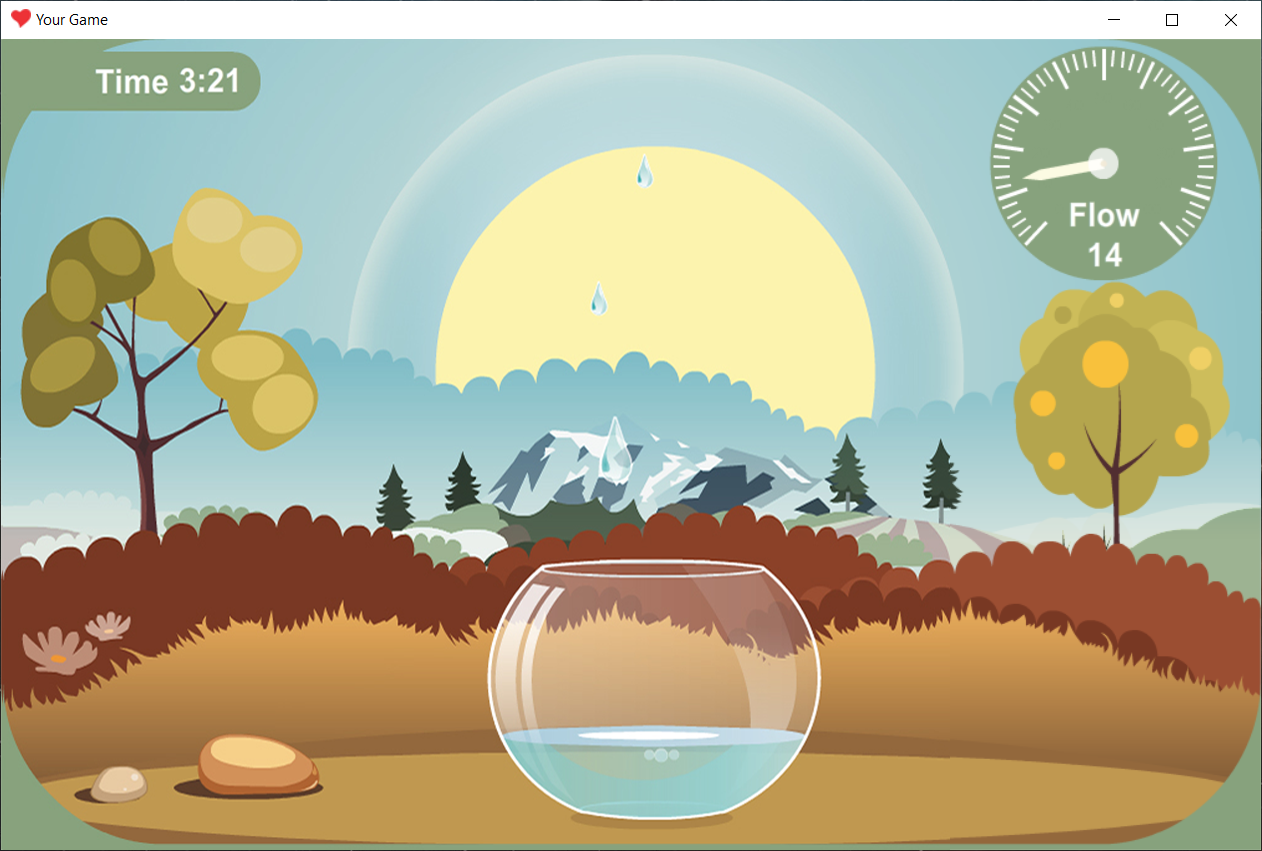
\includegraphics[width=0.75\linewidth]{Images/crystal-clear.png}
    \caption{"You control water. See how different droplets appear as you change the focus level of your brain. The clearer the mind, the larger the drops and the quicker the bowl gets filled. See how quickly can you complete this task using only the power of your mind?".}
    \label{fig:crystal-clear}
\end{figure}

\textbf{Energy Booster}
\begin{figure}[H]
    \centering
    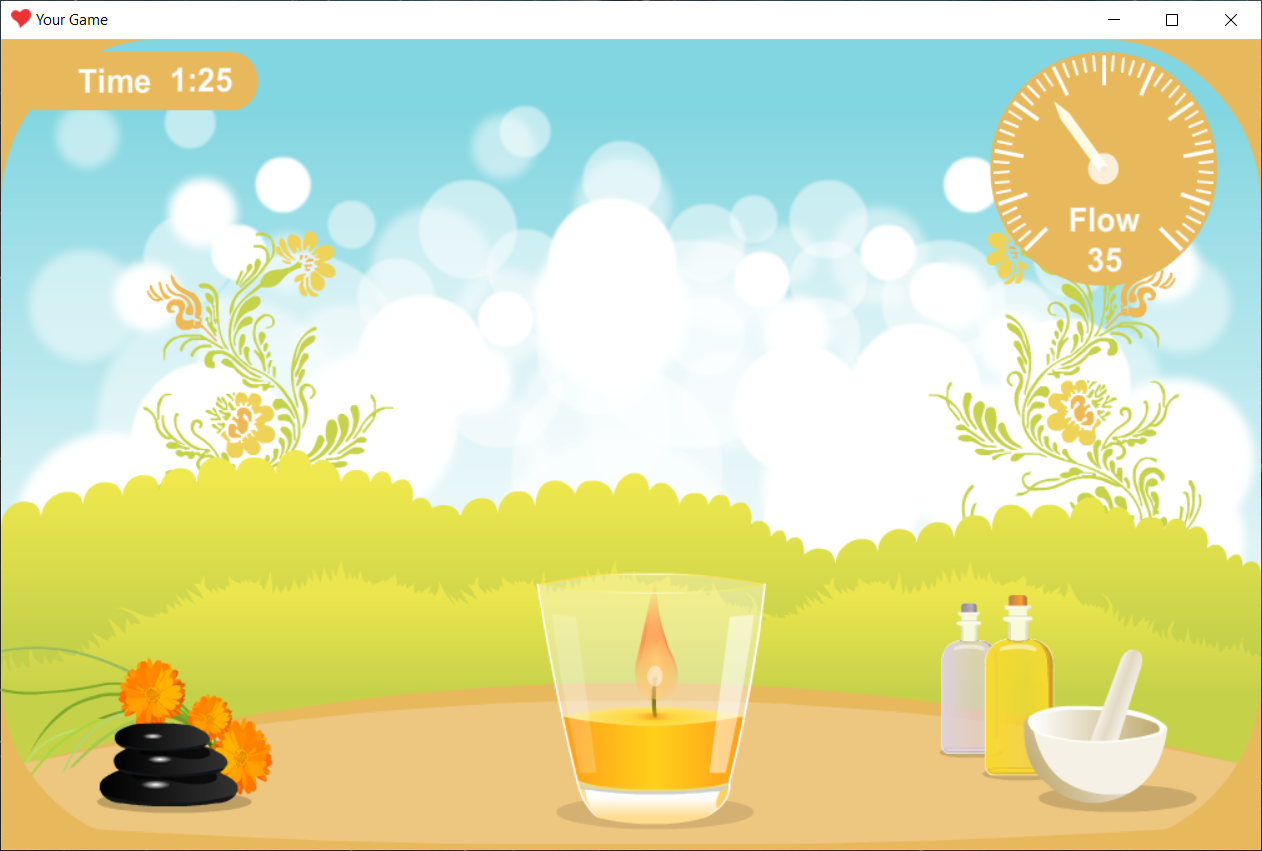
\includegraphics[width=0.75\linewidth]{Images/energy-booster.png}
    \caption{"This game will teach you how to get rid of irritating thoughts, concentrate and focus on what's important now. In order to win, you must repress unnecessary thoughts and emotions (I will show you how). Focus on sensing the here and now. Unlock natural resources in your body to fight fatigue and find energy to do the things you love…"}
    \label{fig:energy-booster}
\end{figure}

\textbf{Instant Relaxation}
\begin{figure}[H]
    \centering
    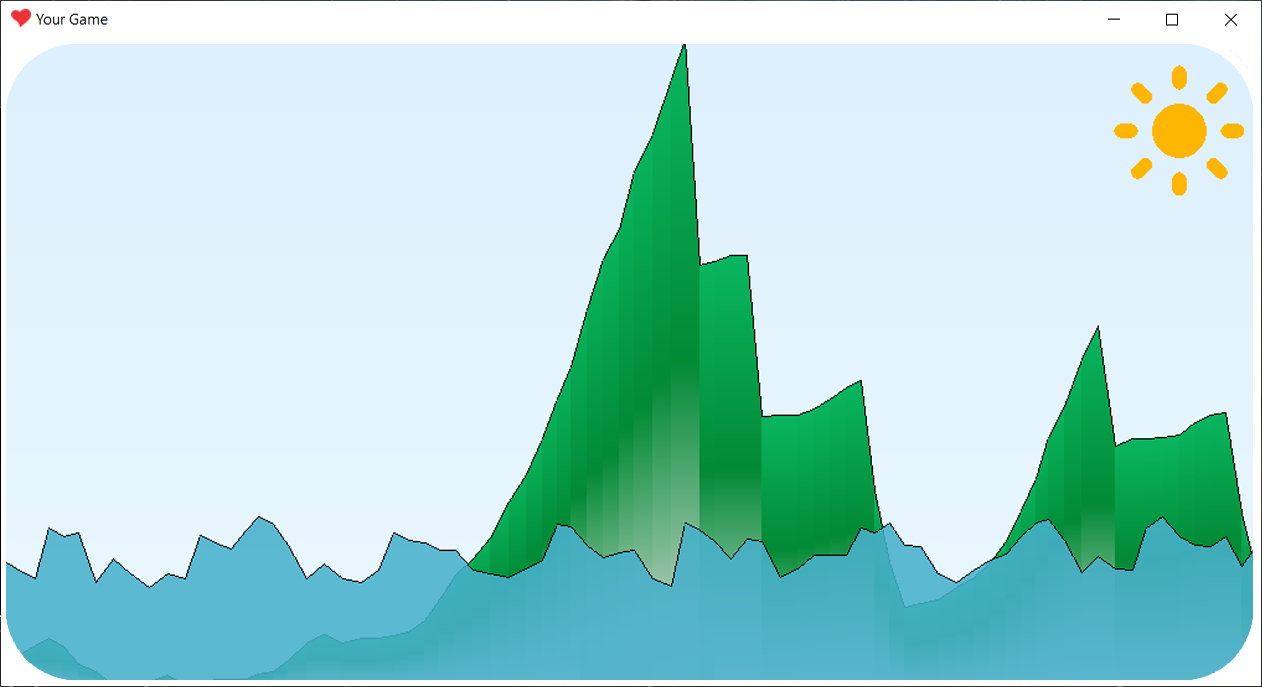
\includegraphics[width=0.75\linewidth]{Images/instant-relaxation.png}
    \caption{"This simple game will train your mind with a powerful technique which will provide instant relaxation. It works is by harmonizing your breathing with your heart rate (HRV). Clear instructions are attached. Even a child can do it! Let this machine work on your mind for one evening… I can guarantee that your friends will gossip about the "Mental Magic" abilities you will be able to show off the next morning."}
    \label{fig:instant-relaxation}
\end{figure}

\textbf{Mental Magic - Mind Control}
\begin{figure}[H]
    \centering
    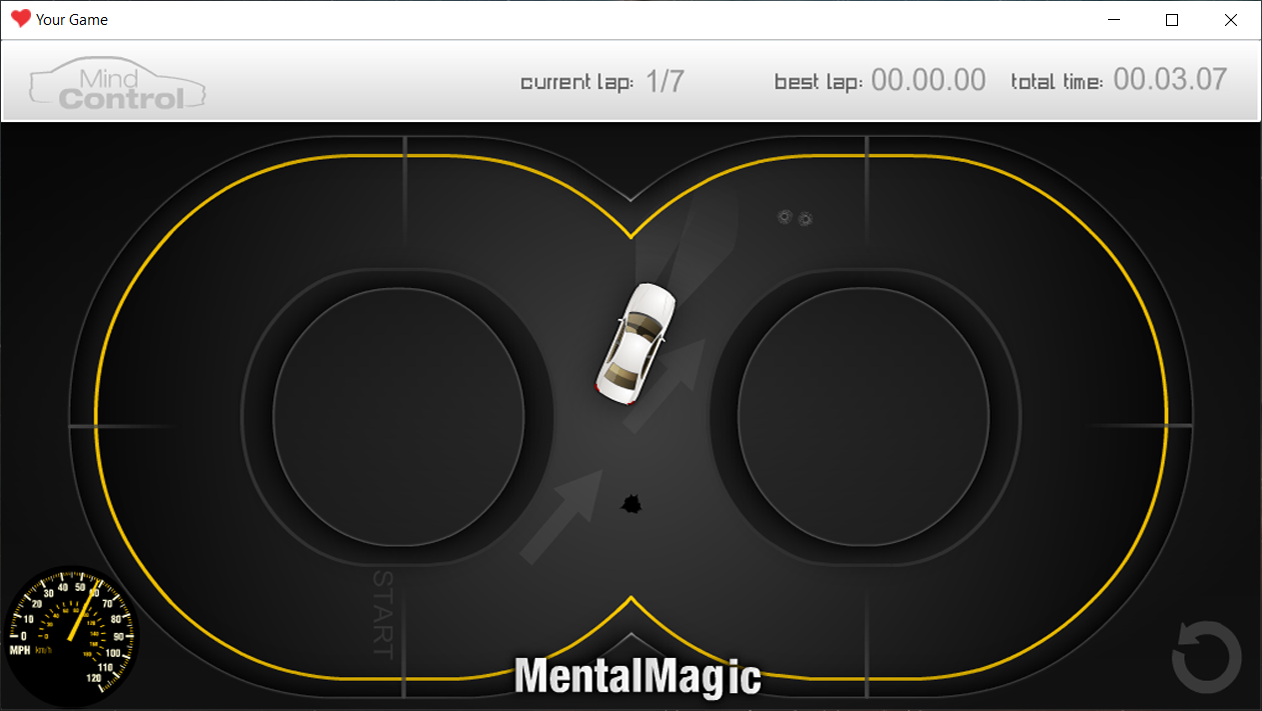
\includegraphics[width=0.75\linewidth]{Images/mental-magic.png}
    \caption{"This game teaches you to control your emotions. In order to complete the task, you must silence your thoughts and emotions. The poorer your mental condition, the harder the game will be to play. The car will move slower and potholes will appear in the road. The better your focus and relaxation, the easier the road will become. The car will gain speed. Test yourself against family members and friends! See who will be the first to complete seven laps."}
    \label{fig:mental-magic}
\end{figure}

\begin{figure}[H]
    \centering
    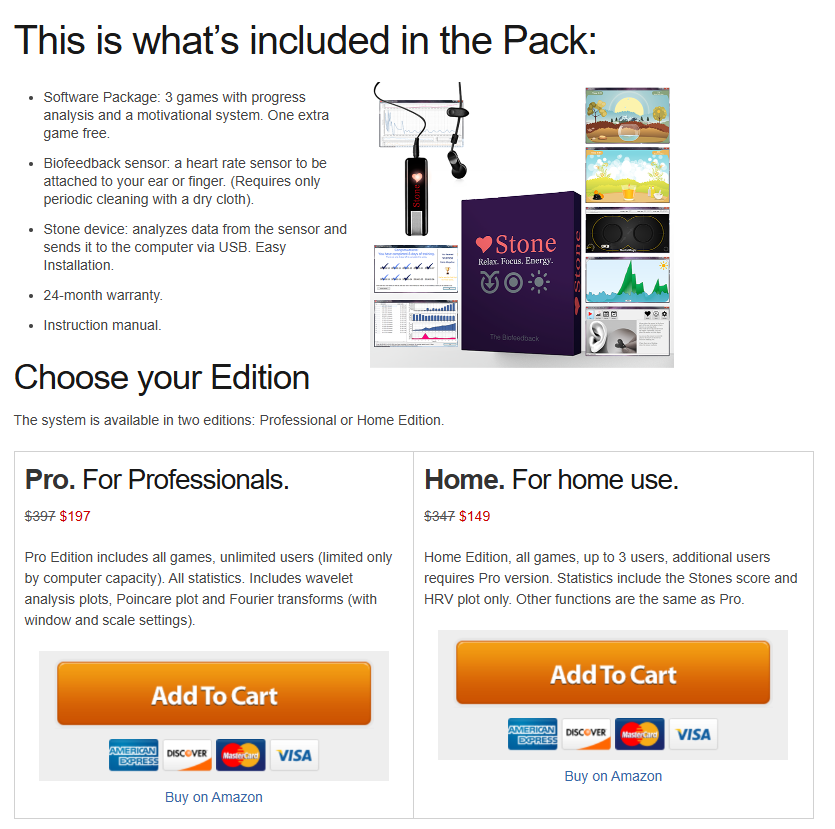
\includegraphics[width=0.7\linewidth]{Images/stone-price.png}
    \caption{A termék ára és a csomag tartalma}
    \label{fig:stone-price}
\end{figure}

\subsection{Miben lesz más ez a projekt?}

A fenti megoldással ellentétben, mi izomaktivitást fogunk mérni két elektromiográf segítségével, ballisztikus (hirtelen) mozgások mérésével, a trifázisos aktivitás mentén képesek lehetünk kiszámolni egy flow értéket \ref{sec:trifazisos}, melynek a maximalizálása lesz a cél a játékunkban és hosszútávon pedig az, hogy képes legyen fejleszteni a játékosok koncentrációs képességeit a mindennapokban is, ennek empirikus bizonyítása túlmutat a szakdolgozatom keretein, ugyanakkor közeljövőbeli célom ennek megvalósítása. 



% todo

\subsection{Kezdő lépések}

Mivel Pythonban szerettem volna a mikrokontrollert vezérelni, ezért a témavezetőmmel úgy döntüttünk, hogy Raspberry pico 2-t fogunk használni micropythonnal. Az ECG modul tökéletes lesz a számunkra, noha mint az később kiderült csak módosítasok után, a modullal járt 3 elektróda, amelyekkel az elektromos aktivitást tudjuk mérni. 


A legelején még csak az ujjmozgató izmok aktivitását néztük, ehhez el kellett helyeznünk egy-egy elektródát az izom kezdő és végpontjában, majd egyet földelés gyanánt a kézfejre tettünk, de ezt bárhová máshová is helyezhettük volna, a mért izmon kívül természetesen. 

A micropython firmware\cite{micropython} telepítését követően, a pico már képes volt python scripteket futtatni, egy egyszerű print utasítással eljutottunk oda, hogy serialba írjon, a chatGPT által írt adatvizualizációs program így már képes volt kimutatni, hogy mit mért az ECG modul.  
\begin{table}[H]
\centering
\begin{tabular}{|l|p{10cm}|}
\hline
\textbf{Termék} & \textbf{Leírás} \\
\hline
\textbf{EKG-01-M} & AD8232 EKG szív monitor modul \\
\hline
\textbf{RPI-PICO-2W} & Raspberry Pi Pico 2 fejlesztői panel, RP2350, Cortex M33, RISC-V, CYW43439 wireless chip \\
\hline
\textbf{RC-40-10/MM} & Szalagkábel csatlakozóval, 10cm, 40p, male-male (jumper) \\
\hline
\textbf{HS-005} & Próbapanel, univerzális NYÁK, forrasztható, 420p, RM2.54mm, 83x54mm \\
\hline
\textbf{AK-300110-010-S} & USB A dugó - micro USB B micro dugó, 1m \\
\hline
\end{tabular}
\caption{Megrendelt termékek listája}
\end{table}


\subsection{Technológiai akadályok}

Már a legelején feltűnt számunkra, hogy nem a várt EMG jelet kapjuk az AD8232-től, ennek elsődleges oka az volt, hogy ez a hardware ECG-re van optimalizálva\cite{AD8232_datasheet}. Itt fontos megjegyezni, hogy az általunk használt ECG modul az valójában a hestore-on vásárolt legális másolata a sparkfun AD8232-nek, a Creative Commons share alike licenszének köszönhetően.\cite{AD8232_datasheet}

így internetes keresést követően azt találtuk, hogy ez a hiba bizonyítottan javítható, bizonyos alkatrészek cseréjével\cite{ecg-to-emg}

Ezek a következők voltak:

\begin{itemize}
    \item 200KOhm fémréteg ellenállás
    \item 27KOhm fémréteg ellenállás
    \item 1MOhm fémréteg ellenállás
    \item 330KOhm fémréteg ellenállás
    \item 100KOhm fémréteg ellenállás
    \item 470nF kerámia kondenzátor
    \item 1nF kerámia kondenzátor
\end{itemize}


A szükséges alkatrészek beszerzését és forrasztási munkálatokat én végeztem.

\begin{figure}[H]
    \centering
    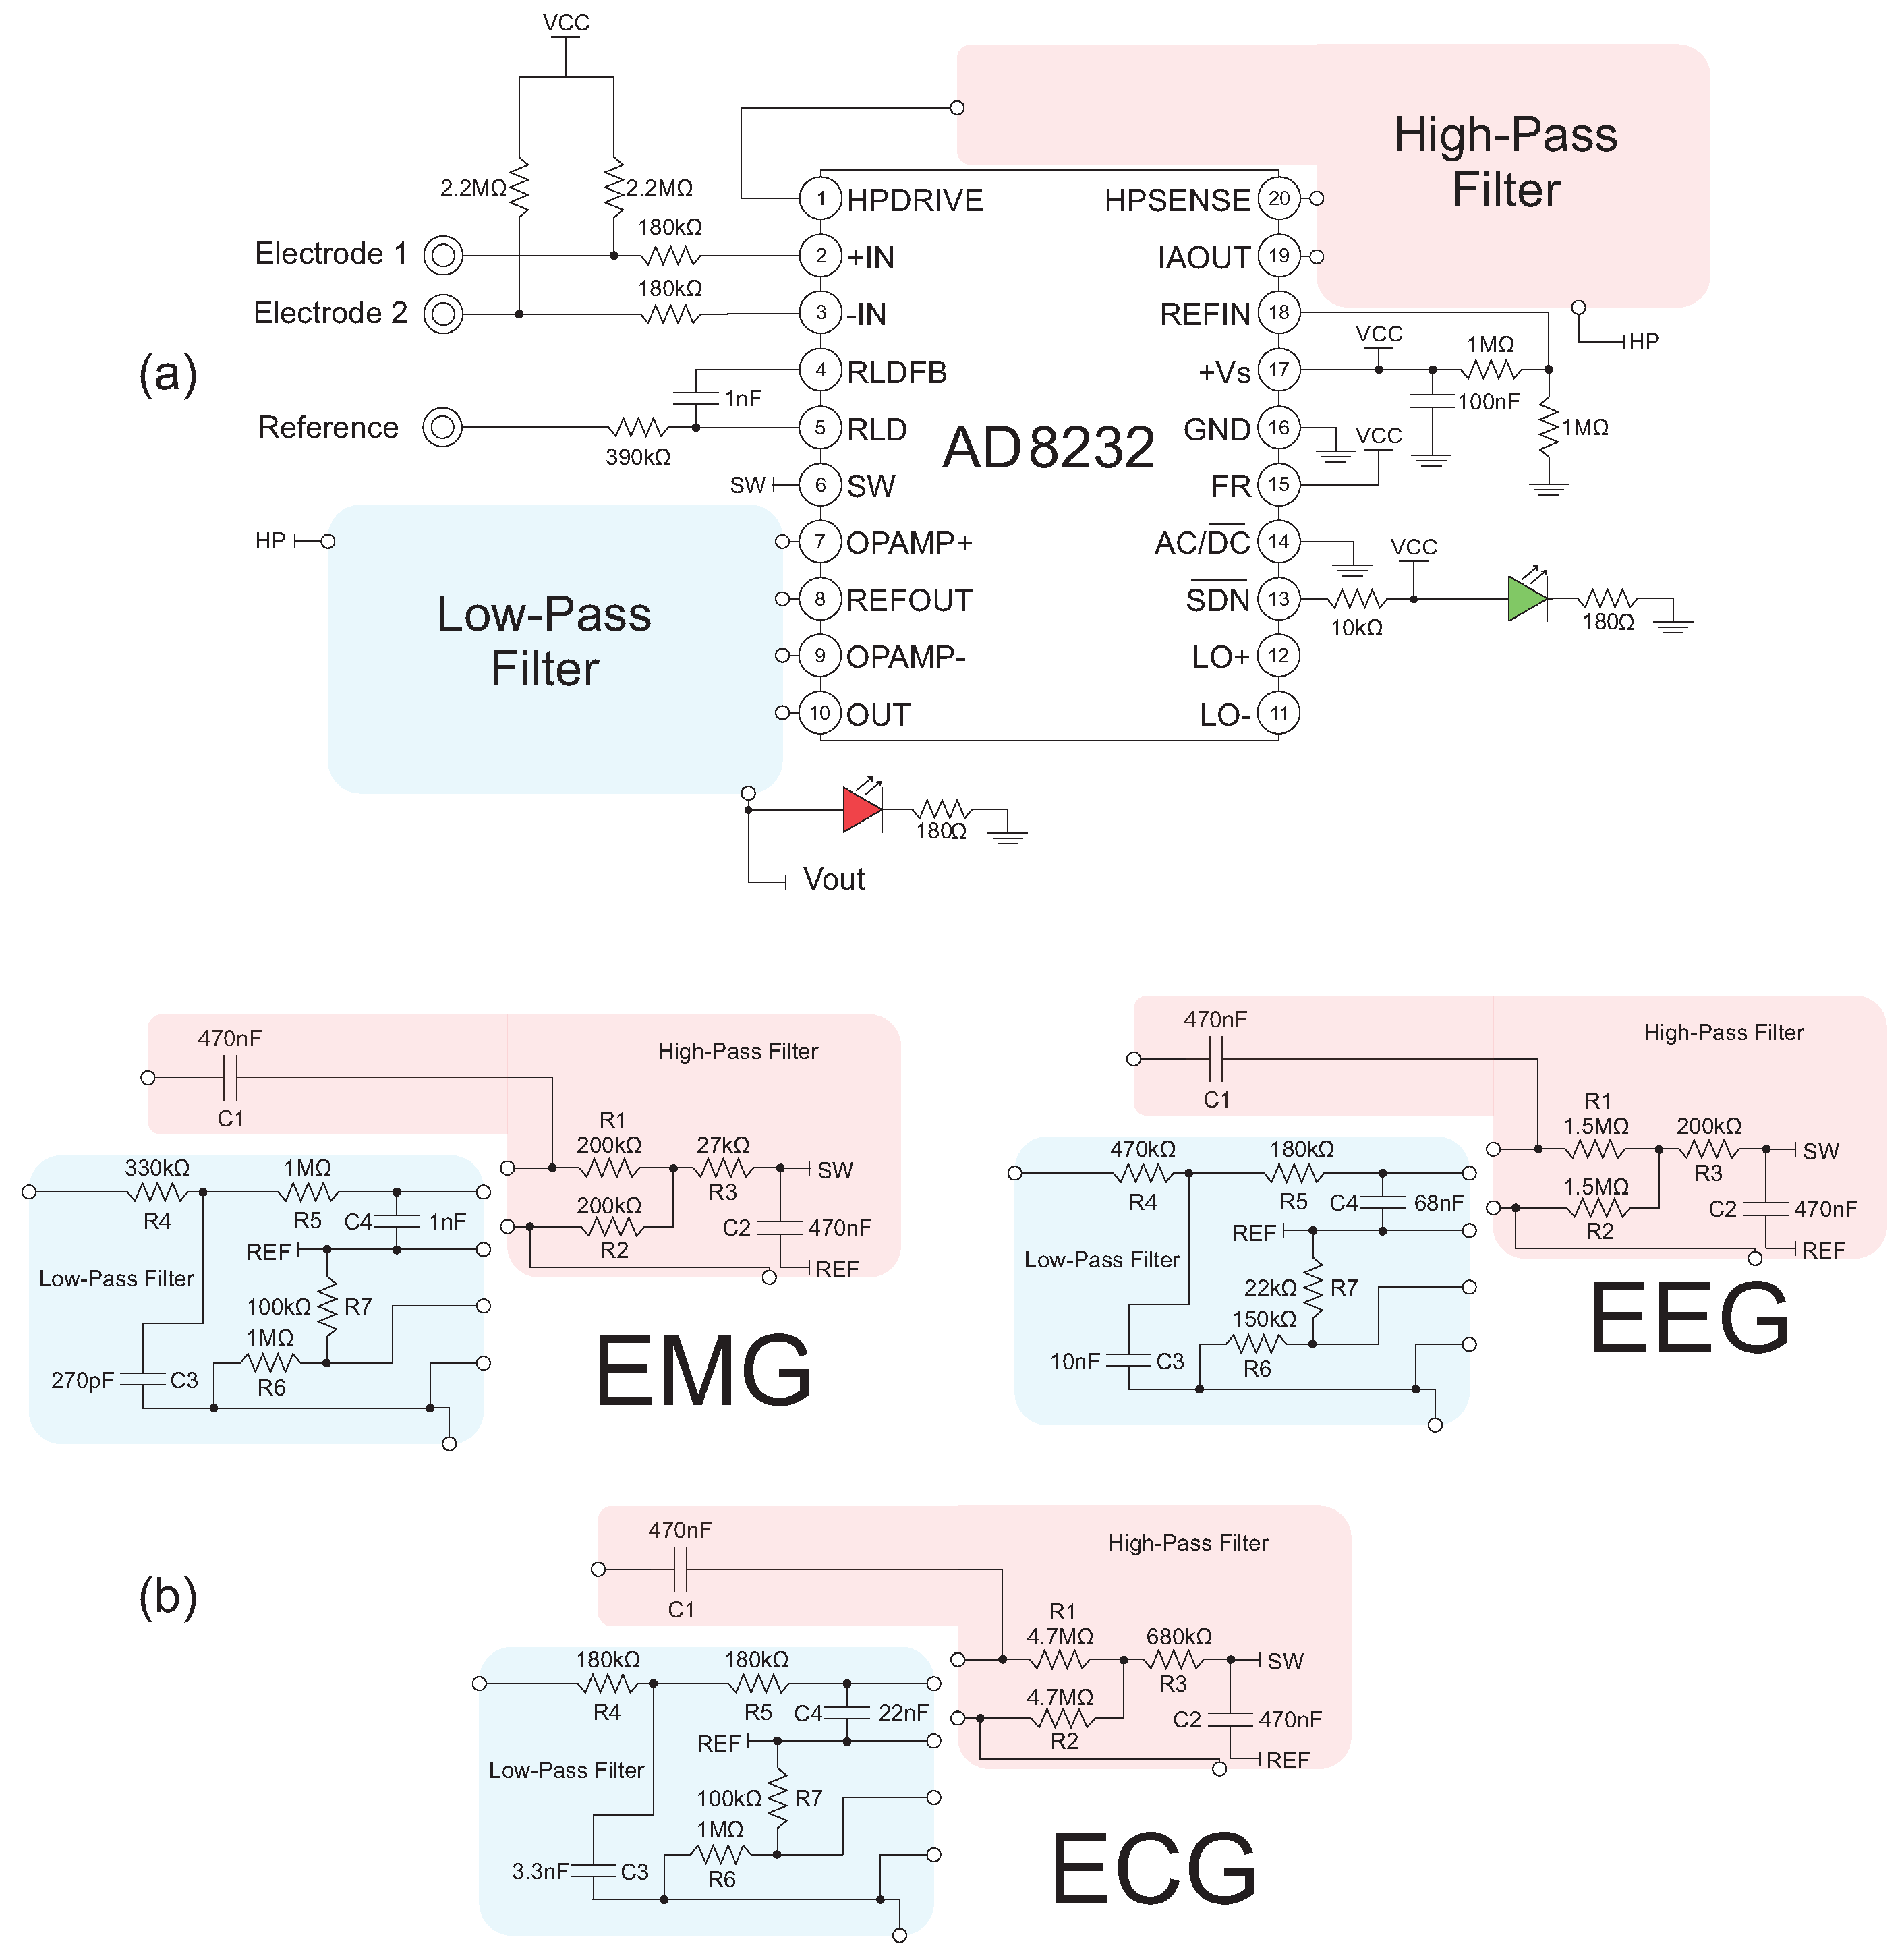
\includegraphics[width=0.7\linewidth]{Images/ecg-to-emg.png}
    \caption{A cikkben leírt megfelelő EMG konfigurációt követtük\cite{ecg-to-emg}}
    \label{fig:good-config}
\end{figure}


\subsection{Adatok továbbküldése a számítógépre\texorpdfstring{ \cite{usb-article-1,usb-article-2,usb-article-3}}{}}
Fontos megjegyeznem, hogy a következő fejezet, a fent említett források összefoglalásából és fordításából született.

Mivel a célunk az, hogy a játékunk dinamikusan igazodjon a felhasználó fiziológiai állapotához, ezért szükségünk van folyamatos kommunikációra a számítógép és a modul között,
erre a legalmasabbnak megoldásnak azt gondoltuk, hogy kontrollerként fogjuk emulálni a pico-t, így a folyamatos jelet képesek vagyunk analógként, vagy éppenséggel ravaszként beállítani, 
a játékunk elsődlegesen kontrollre lesz tervezve. 

\subsubsection{Universal Serial Bus (USB)}
Az USB az egyik legelterjedtebb vezetékes kapcsolódási forma a számítógép és valamilyen eszköz között, 1994 előtt a számítógépek egyik nagy hiányossága volt, hogy számtalan különféle csatlakozási módot használtak, ilyen volt pl. a VGA, PS2 portok is, amiből több féle is volt.
Ez problémás volt, hiszen ha az egér PS2-es portjába billentyűzetet csatlakoztatott véletlenül valaki figyelmetlenségből, akkor az operációs rendszer nem ismerte fel az eszközt.

1994-ben a Compaq, DEC, IBM, Intel, Microsoft, NEC, és Nortel közös erőfeszítésével megalkották a ma ismert USB architektúrát, amely képes volt svájci bicskaként működni az informatikában, ami a csatlakozókat illeti és nem mellesleg gyorsabb is volt mint az addigi megoldások.

\subsubsection{USB architektúra}
Az USB egy aszinkron protokol, ami a mester-szolga architektúrára épül, ugyanakkor csak egy host lehet egy rendszeren belül és minden kommunikáció az eszközökkel csak a host kezdeményezésére 

Egy host két részből áll:

\begin{itemize}
    \item Host controller: ez felel az új eszközök felismeréséért, kezeléséért
    \item Root Hub: hardveres elem, ami központi belépési pontja az USB eszközöknek
\end{itemize}

Minden csatlakoztatott eszköznek van egy címe, amivel a host eltudja érni. A host 127 kapcsolatot képes kezelni,  azért csak ennyit mert az UBS protokol 7 bites címekre van korlátozva.

\subsubsection{USB sebessége}

Az USB specifikáció megkülönböztet sebbesség kategóriákat:

\begin{itemize}
    \item Low-Speed devices (maximum 1.5Mb/s); ide tartoznak az egerek, billentyűzetek
    \item Full-Speed devices:  (maximum 12Mb/s); USB támogatott mobil telefonok, audio eszközök
    \item High-Speed devices:  (maximum 480Mb/s); pendriveok, külső tárolók
    \item Super-Speed(+) devices:  (maximum 20-80Gb/s); 
\end{itemize}

\subsubsection{USB végpontok}

Egy USB eszköz, végpontokat tartalmaz, egy végpont az eszköz önállóan hivatkozható részét jelöli, ami képes információ közvetítésre a host és az eszköz között. Fontos megjegyezni azt, hogy ezen címek egyedisége csak az eszközön belül áll fenn. 

A végpontok úgynevezett, pipeokkal vannak hozzákötve a bufferhez.


\begin{figure}[H]
    \centering
    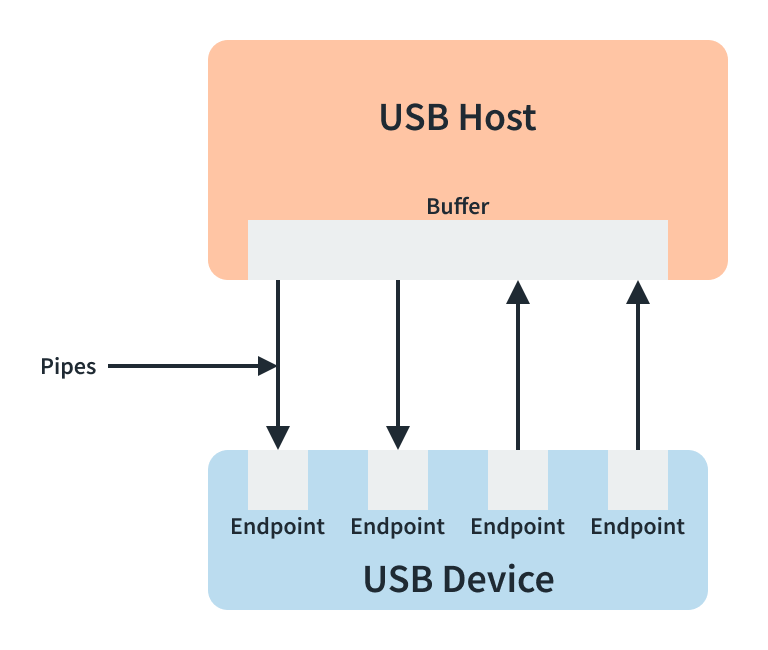
\includegraphics[width=0.7\linewidth]{Images/usb-figure-2-1.png}
    \caption{USB data flow model\cite{usb-article-2}}
    \label{fig:usb-data-flow}
\end{figure}

Az USB végpontok egyirányúak és az adat csak olyan irányba áramolhat, amelyet a végpont megenged. leggyakrabban ciklikus redundancia vizsgálatot használnak a hibák keresésére (Cyclic Redundancy Checks - CRC). Ez a módszer checksum számítás követően hozzzáfűzi a csomaghoz ezt az értéket, majd a fogadó fél újra kiszámolja a checksumot, amennyiben a két checksum egyezik, sikeres volt az adatátvitel.

A végpontokra azért van szükség, mert az eszközöknek eltérhet a mintavételezési rátája, ahogy az adatmennyiség is egy csomag esetén.

\subsubsection{kommunikáció}

A kommunikáció az USB 2.0 esetében félig duplex, mivel továbbítás és fogadás egyszerre nem valósítható meg, a tranzakciókat a host indítja és a hubhoz kapcsolódó eszközök, csak válaszolni tudnak rá.

Amennyiben megnézzük az USB protokolt az idő szempontjából, egy frame sorozatot tartalmaz. Egy frame rendelkezik egy start of frame (SOF) csomaggal és egy vagy több tranzakcióval. 

\begin{figure}[H]
    \centering
    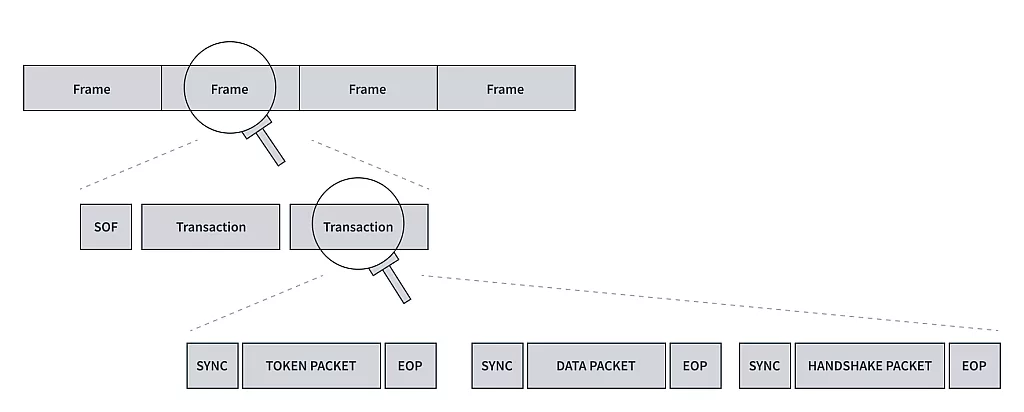
\includegraphics[width=0.7\linewidth]{Images/usb-figure-2-2.png}
    \caption{USB frame\cite{usb-article-2}}
    \label{fig:usb-frame}
\end{figure}

Az ábra megmutatja, hogy egy tranzakció egy token csomagból, opcionális adatcsomagból és handshake csomagból áll. 

Egy csomag tartalmazhat:
\begin{itemize}
    \item Packet ID (PID) - azonosítás
    \item Optional Endpoint Address - 4 bites cím
    \item Optional Payload Data - továbbítandó adat egy kis része (0 - 1023 byte)
    \item Optional CRC - hibavizsgálat
\end{itemize}

\subsubsection{Tranzakciók}

\paragraph{1. Token csomagok}


A token csomagokat, mindig a host küldi és a forgalom irányításáért felelősek. A token csomag adja meg a tranzakció típusát.

Ez a csomag így alakul:
\begin{itemize}
    \item Packet ID (PID)
    \item 7-device address
    \item 4-bit endpoint ID
    \item 5-bit CRC
\end{itemize}

Három különböző változata van:

\begin{itemize}
    \item IN token packet - kérés az eszközről a hostnak
    \item OUT token packet - megerősítés, a host eszközről, hogy készen áll a küldésre
    \item SETUP token packet - konfigurációk és beállítások során kerül küldésre 
\end{itemize}

Van egy token csomag típus, amit érdemes külön is említeni, ez az úgynevezett Start of Frame (SOF) csomag, ez egy olyan speciális csomag, ami tartalmaz egy 11-bites frame number nevű mezőt, ami mutatja a jelenlegi és eddig elküldött csomagok számát. A frame number mindig inkrementálódik, amikor megjelenik egy új SOF az adatsinen.

\paragraph{2. Adatcsomagok}


Ezek a csomagok tartalmazzák, a továbbítandó adatnak egy részét.

Fontos, hogy ezek kétféle ID-val rendelkezhetnek, ID0-val és ID1-el, Ennek hibavizsgálati okai vannak, mivel az adatcsomagok esetében, a küldők alternálják ezeket, így ha két azonos ID-vel ellátott csomagott kapunk egymás után, akkor biztosra vehetjük, hogy beszélhetünk adatveszteségről.


\paragraph{3. Handshake csomagok}


Ezeket a csomagokat a csomagokat a tranzakciók zárására használjuk.
Mindig a tranzakciót fogadó fél küldik ki ezeket.

Lehetnek:

\begin{itemize}
    \item ACK - sikeres továbbítás
    \item NAK - sikertelen továbbítás
    \item STALL - hibajelzés
    \item NYET - A fogadó fél még nem áll készen a csomag fogadására (Csak High-Speed eszközök esetén) 
\end{itemize}

\paragraph{4. Különleges csomagok}


\begin{itemize}
    \item PRE - hubok számárá küldi ki a host, jelezve hogy a következő csomag low-speed lesz (Csak Full/High-Speed eszközök esetén)
    \item PING - NYET csomag beérkezése után, ellenörzi az eszköz elérhetőségét (Csak High-Speed eszközök esetén)
\end{itemize}

\paragraph{Tranzakciók típusai}


\begin{itemize}
    \item Upstream/Read/IN - Olyan tranzakciók, melyeket az eszközről küldünk a hostnak. A tranzakciót a host kezdeményezi, hogy adatot kérhessen egy IN csomaggal rendelkező eszköztől. Amennyiben az eszköz nem képes adatot fogadni egy NAK-el fog válaszolni, majd később újra próbálja. Sikeres adatfogadás esetén egy handshakkel zárul.
    \item Olyan tranzakciók, melyeket a hostról küldünk az eszköznek. A tranzakciót a host kezdeményezi, hogy adatot küldhessen egy OUT csomaggal rendelkező eszköznek. Amennyiben az eszköz nem képes adatot fogadni egy NAK-el fog válaszolni, majd később újra próbálja. Sikeres adatfogadás esetén egy handshakkel zárul.
    \item Control - Segít beazonosítani, beállítani, irányítani az eszközöket és lehetővé teszi a host számára hogy adatokat olvasson ki az eszközről, beálíthassa az eszköz címét, 
\end{itemize}

\subsubsection{Descriptorok}

Az USB Descriptorok személyigazolványként működnek az eszközök számára, hasonlóak a egy használati utasításhoz.

\paragraph{Device Descriptor}


Amikor csatlakoztatjuk az eszközt. az első kérése a hostnak a device descriptor. Ez biztosítja a host számára az összes szükséges információt, amire szüksége van, hogy megfelelően tudja kezelni az eszközt. 


\paragraph{Configuration Descriptor}


A configuration descriptor megadja hogy hogyan kommunikáljunk a host rendszerrel, például megadhatjuk az interfészek számát

\paragraph{Interface Association Descriptor (IAD)}


Az IAD célja, hogy több interfészt csoportosítva egy funkcionáló egységet alkosson belőlük. A kezdeti fázisban az USB specifikációk nem támogatták a multi-interface funkciókat, ezért született meg az IAD.

\paragraph{Interface Descriptor}


Az interface descriptor egy olyan adatszerkezet, ami végpontok gyűjteményének is nevezhető egy USB eszközön belül.

\paragraph{Endpoint Descriptor}


Ez a descriptor alapvető információt tartalmaz egy konkrét végpontról. Minden végpontnak saját adat csatornája van, lehet az IN vagy OUT. 

\paragraph{String Descriptor}


Ez a descriptor emberek számára is érthető módon írja le az USB eszköz tulajdonságait. Opcionális, de erősen ajánlott, több nyelv esetében, több string descriptorra van szükségünk.


\subsubsection{USB Enumeration and Configuration}

Három fázisra bontható:

\begin{itemize}
    \item Dynamic Detection - az USB sebességét ismeri fel a csatlakozást követően
    \item Enumeration and configuration A host elkéri a device descriptort, ahonnan megtudja a maximális csomag mennyiséget, ezt követően a host újra indítja az eszközt és új címet ad neki, majd elkéri maradék descriptorokat is, ha ez is megvan, a host betölti a drivert.  
    
\end{itemize}Lehetnek:


\subsubsection{USB osztályok}

A szabványosított osztályok a következők:

\begin{itemize}
    \item HID (Human Interface Device) - képessé teszi a felhasználót arra, hogy kommunikáljanak a számítógéppel, mint például az egér, billentyűzet, kontroller.
    \item USB Mass Storage - pl. külső HDD
    \item USB Video - pl. kamerák
    \item USB Printer
    \item USB Communication Device Class (CDC)
\end{itemize}

\subsubsection{HID fogalma}
A hardverünkön CircuitPython fut, ez 3 különböző HID eszközt tud emulálni, egeret, billenytyűzetet és úgy nevezett consumer controlt\cite{customising-devices,custom-hid}



A pico emulált kontroller descriptora így néz ki. \cite{customising-devices}

itt beszélek \aref{fig:desc}. ábráról

\begin{lstlisting}[language=Python]
         GAMEPAD_REPORT_DESCRIPTOR = bytes((
    0x05, 0x01,  # Usage Page (Generic Desktop Ctrls)
    0x09, 0x05,  # Usage (Game Pad)
    0xA1, 0x01,  # Collection (Application)
    0x85, 0x04,  #   Report ID (4)
    0x05, 0x09,  #   Usage Page (Button)
    0x19, 0x01,  #   Usage Minimum (Button 1)
    0x29, 0x10,  #   Usage Maximum (Button 16)
    0x15, 0x00,  #   Logical Minimum (0)
    0x25, 0x01,  #   Logical Maximum (1)
    0x75, 0x01,  #   Report Size (1)
    0x95, 0x10,  #   Report Count (16)
    0x81, 0x02,  #   Input (Data,Var,Abs,No Wrap,Linear,Preferred State,No Null Position)
    0x05, 0x01,  #   Usage Page (Generic Desktop Ctrls)
    0x15, 0x81,  #   Logical Minimum (-127)
    0x25, 0x7F,  #   Logical Maximum (127)
    0x09, 0x30,  #   Usage (X)
    0x09, 0x31,  #   Usage (Y)
    0x09, 0x32,  #   Usage (Z)
    0x09, 0x35,  #   Usage (Rz)
    0x75, 0x08,  #   Report Size (8)
    0x95, 0x04,  #   Report Count (4)
    0x81, 0x02,  #   Input (Data,Var,Abs,No Wrap,Linear,Preferred State,No Null Position)
    0xC0,        # End Collection
))
        \end{lstlisting}

\section{A trifázisos izommozgás}
\label{sec:trifazisos}

Az alábbiakban be fogom mutatni a trifázisos izommaktivációs mintázatot, hogyan mérhető EMG-vel és hogyan segíthet flow-ba kerülni.


\section{A ballisztikus mozgás}
A ballisztikus mozgás, gyors előre programozott mozdulat, mely a visszajelzés előtt befejeződik.

\section{A mozgás 3 fázisa}
 \begin{enumerate}
     \item Aktivitás az agonista(AG1) izomban, gyorsítja a végtagot.
     \item Aktivitás az antagonista(ANT) izomban, a fékezésért felelős.
     \item Aktivitás az agonista(AG2) izomban, a stabilizálásért felel.

     Ezek a fázisok és erősségeik nem konstansok, vagyis hatással van rájuk a hangulatunk, az adott feladat \cite{triphasic-movement-is-influenced-by-situational-factors}. 
 \end{enumerate}

\begin{figure}[H]
\centerline{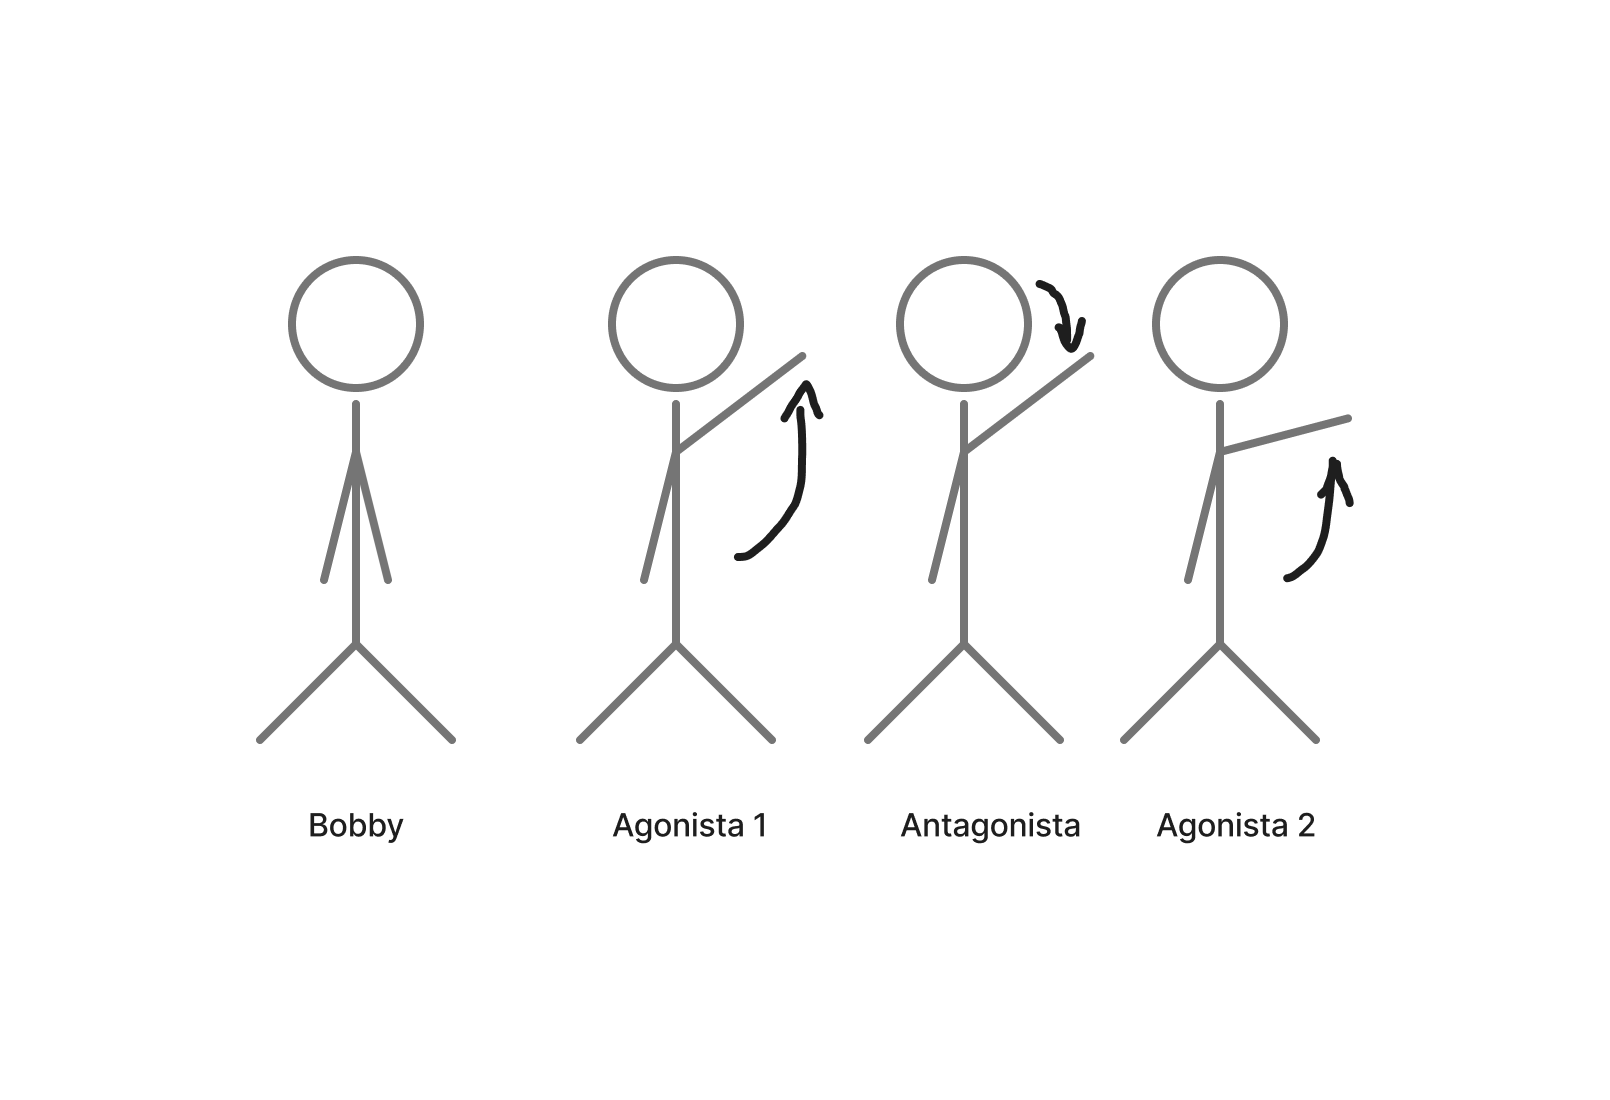
\includegraphics[width=\linewidth]{Images/bobby_trifazisos.png}}
\caption{Trifázisos izommozgás példa.}
\label{fig:trifazisos}
\end{figure}

\section{A gyakorlás hatása}

Az elterjedt gondolat az, hogy az izommozgás precizitása a sebességgel fordítottan arányos,  ez valóban igaznak látszik, ugyanakkor ennek a negatív korrelációnak a csökkenését nevezhetjük fejlődésnek, pontosan ez történik a gyakorlás hatására. 

Az amplitúdók ingadozása csökkent a gyakorlása hatására és a maximális sebességig való eljutás és megtartása konstans maradt.\\

A teljesítmény javulása az agonista, antagonista izommozgások időbeli változásának köszönhető, mikor a maximális gyorsaság nem változott semmit sem.
\cite{improvement-in-ballistic-movement}

\section{A két elmélet}
Az egyik elmélet azt mondta ki, hogy a mozgásban való ilyen módú fejlődés az annak köszönhető, hogy az agyunk egy erősebb jelet küld mint előtte AG1-ként. 

A másik elmélet szerint rövidülnek az impulzusok ezáltál növelve a teljesítményt, végül ahogy ez a kutatás is bizonyította nyert ez a nézőpont\cite{improvement-in-ballistic-movement}.

\section{A flow állapota}

A flow fogalmát Csikszentmihályi Mihály vezette be először a köztudatba \cite{cziksentmihalyi1990flow}. A flow állapot egy optimális mentális állapot, amelyben az egyén teljesen elmerül a tevékenységében, és a cselekvés és a tudatosság egybeolvad.

Úgy is mondhatjuk, hogy a flow alatt olyan optimális élményeket értünk, amelyek a legélvezetesebbek az emberi életben. 

Kijelenthetjük azt is, hogy aki többször van flowban az boldogabb és elégedettebb is.

\subsection{A flow állapot jellemzői}

A flow állapot több kulcsfontosságú jellemzővel bír:

\begin{itemize}
    \item \textbf{Elveszett időérzék}: Az időérzékelés megváltozik, az idő gyorsabban vagy lassabban telni látszik.
    \item \textbf{Teljes koncentráció}: Az egyén teljesen elmerül a tevékenységben, a külvilág háttérbe szorul.
    \item \textbf{Optimális stressz szint}: A feladat nehézsége és a személy képességei egyensúlyban vannak, ami facilitáló hatású.
    \item \textbf{Magas teljesítmény}: A flow állapotban az egyén csúcsteljesítményre képes.
    \item \textbf{Belső motiváció}: A tevékenység önmagáért motiváló, külső jutalom nélkül is.
    \item \textbf{Egyértelmű célok és azonnali visszajelzés}: A feladat világos célokat tartalmaz, és a visszajelzés azonnal érkezik.
\end{itemize}

\subsection{A flow és a trifázisos izommozgás kapcsolata}

A flow állapot eléréséhez elengedhetetlen a hatékony motoros kontroll. A trifázisos izommozgási mintázat optimalizálása során \cite{improvement-in-ballistic-movement} hozzájárulhat a flow állapot elérésének megkönnyítéséhez, mivel:

\begin{itemize}
    \item A mozgások automatizálódnak, csökkentve a kognitív terhelést
    \item A precíz izomkontroll lehetővé teszi a feladatra való teljes koncentrációt
    \item Az optimalizált mozgásminták növelik az önbizalmat és a kontroll érzését
    \item A hatékony motoros végrehajtás lehetővé teszi a magasabb szintű célokra való fókuszálást
\end{itemize}

\subsection{A flow mérése}
A flow-t, általában kérdőívekkel mérik, introspekció alapján, ezzel az a gond, hogy az emberek eltérően értelmezhetik ugyanazt a kérdést, nyilatkozhatnak úgy is, hogy az nem feltétlenül fedi az objektív valóságot, hiszen az introspekció alapú kérdőívek pontossága, korrelál az egyén önismeretével, ami szintén nem egy objektív kvantifikálható érték.\cite{methodological-limitations-of-introspections-in-ageing-studies, The-Introspection-Illusion} Ezen okokból sok kritika éri a pszichológia tudományát, ugyanakkor egyre inkább haladunk az objektív mérések felé, ez itt sincs másképp. Az EMG más néven Elektromiográfia, az izmok neurális aktivációját hivatott mérni, mi 3 elektródával végezzük mindezt, de a trifázisos izommozgáshoz 5 darab fog kelleni, hiszen kell két elektróda az Agonista izom kezdő és végpontjaiba, majd kettő az Antagonista izom kezdő és végpontjaiba és végül a kontrol elektróda egy semleges helyre, ez nálunk a kézfej szokott lenni.

Mostmár tudjuk azt, hogyan mérhető EMG-vel a trifázisos izommozgás, de hogy jön képbe a flow? A flow állapota korrelál a nagyobb ballisztikus mozgás precizitással.

 A ballisztikus mozgások során megfigyelhető trifázisos mintázat (AG1, ANT, AG2) optimalizációja jelzi ezt a fejlett állapotot. A kutatások szerint a gyakorlott, precíz mozgásnál – amennyiben a maximális sebesség állandó – az izomaktivitás időzítése megváltozik: az AG2 (második agonista löket) időtartama lerövidül és a megjelenése korábbra tolódik,. Ez a temporális finomhangolás teszi lehetővé a pontosabb megállást és a mozgásvariabilitás csökkenését, amely a flow-élmény fiziológiai kísérőjelensége lehet.

 \section{Kísérleti Módszertan és Jelfeldolgozás}

A kutatás során célunk egy objektív mérőszámrendszer kialakítása, amely képes valós időben vagy utólagos elemzéssel kimutatni a trifázisos mintázat finomhangolását a ballisztikus ujjmozgások során.

\subsection{Mérési elrendezés}
A mérésekhez felületi EMG (sEMG) szenzorokat alkalmazunk. Mivel az ujjak finommotorikus mozgatásáért felelős izmok hasa az alkaron található, az elektródákat itt helyezzük el. A vizsgált mozgás egy gyors, ballisztikus ujjextenzió (ujj felemelése) és flexió (leütés), amely jellemző a gépelésre vagy hangszeres játékra.

Az 5 elektróda elhelyezése a következő anatómiai pontokon történik:
\begin{enumerate}
    \item \textbf{Agonista (AG):} Biceps Brachi - a tenyér kiforgatásáért felelős izom
    \item \textbf{Antagonista (ANT):} Pronator Teres - a tenyére befele forgatásáért felelős izom
    \item \textbf{Referencia:} Semleges pont a csuklócsont felett (Processus styloideus ulnae), ahol nincs izomaktivitás.
\end{enumerate}


\section{Várt Eredmények és Hipotézisek}

A szakirodalom és az elméleti háttér alapján a következő összefüggéseket feltételezzük a mért adatokban, amikor az alany eléri a flow állapotot:

\begin{enumerate}
    \item \textbf{ANT fázis precizitása:} Flow állapotban az antagonista izom (Flexor) fékező hatása (ANT burst) élesebben elkülönül, minimalizálva az ujj felesleges rezgését a billentyű/felület elérésekor.
    \item \textbf{Kokontrakció csökkenése:} Kezdőknél vagy stressz alatt gyakori, hogy a feszítő és hajlító izmok egyszerre feszülnek (merev kéz). Flow állapotban ez az átfedés minimalizálódik, az izmok "átadják" egymásnak a munkát.
    \item \textbf{AG2 redukció:} A gyakorlottság hatására a mozgás végén lévő korrekciós feszítés (AG2) amplitúdója csökken, jelezve a hatékonyabb neurális vezérlést.
\end{enumerate}

\section{Mérés a gyakorlatban}

Amint megérkezett a második ECG modul és átalakítottuk EMG-vé, akkor bele is vágtunk a mérésbe, az ujjmozgató izmok trifázisos aktivitását szerettük volna mérni. Az alábbi eredmények oszcilloszkóp segítségével történtek, ahol két mérőfejet használtunk, ezek földelése a gnd-hez volt bekötve, míg a mérócsúcsök a két analóg kimenetre. A mérőeszköz használata lehetőve tett még a pico2-nél is egy pontosabb mérést. Az eredmények összefoglalója ezen a képen látható:

\begin{figure}[H]
\centerline{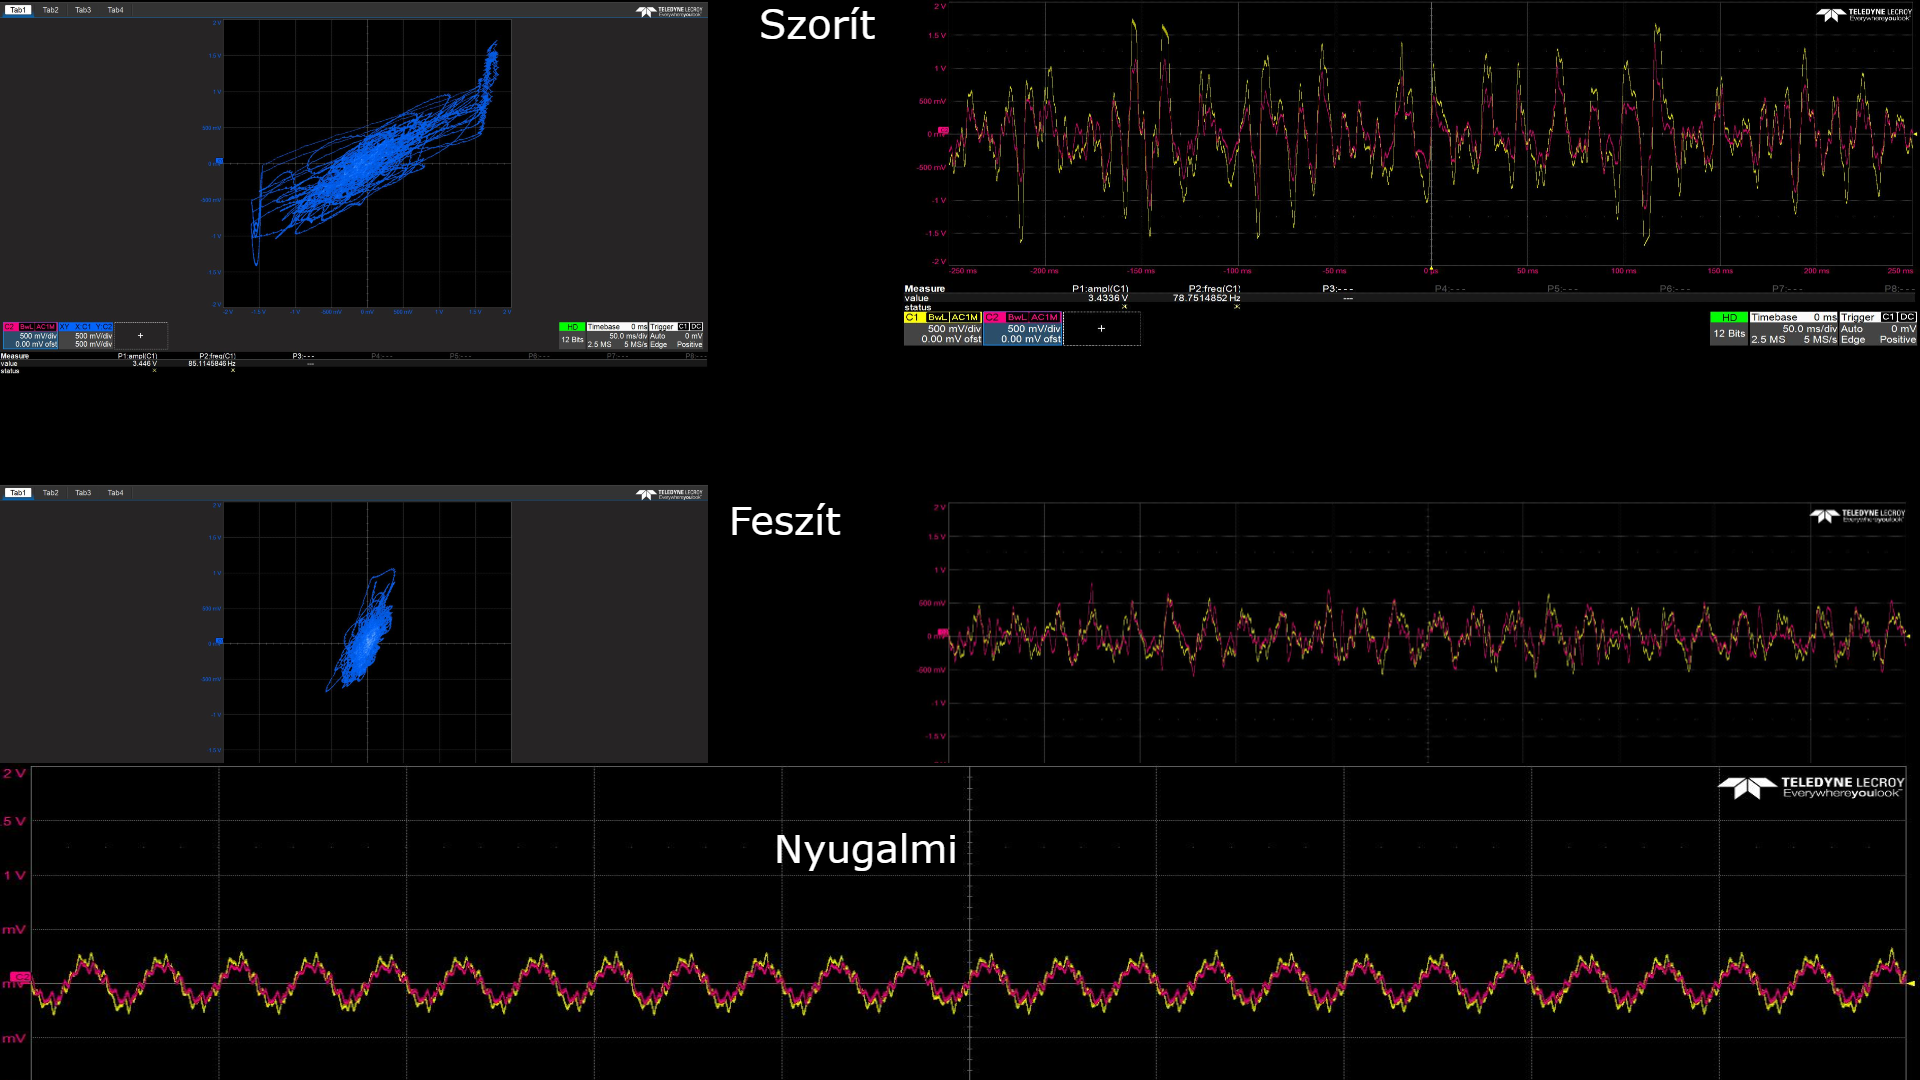
\includegraphics[width=\linewidth]{Images/összevetés.png}}
\caption{Az EMG mérés eredményeinek összefoglalója.}
\label{fig:osszevetes}
\end{figure}

A kép baloldalán láthatóak a korrelációk az agonista és az antagonista izmok között, míg a többi képen a mért értékek egymásra illesztését láthatjuk. Ami tisztán látható, hogy a feszítő és szorító korrelációok eltérnek egymástól és ezeknek a vizulizációjában láthatjuk azt, hogy szinte ugyanolyan utat jár be mindkét jel. Ez gyanús volt számunkra, arra gyanakodtunk hogy túl nagy az interferencia hiszen a felvétel során mind az 5 elektródának közel kellett lennie egymáshoz az alkaron. Az is felmerült bennünk, hogy a ballisztikus mozgások hiánya okozhatja ezeket a furcsaságokat. 

Ugyanebben a periódusban jöttünk rá, hogy a fékezés aktivitása problémás lehet olyan mozgások esetében ahol fenn áll egy ütközés, hiszen akkor megtörténhet mondjuk kontroller esetében hogy az analógot mindig ütközésig nyomja valaki, így egyáltalán nem vagy kevésbé kell fékeznie a felhasználónak az izommozgást. 

Ezt követően beszélgettem egy orvosis barátommal \pageref{sec:koszonet}, aki új ötleteket adott. Egyrészt elmondta, hogy nincs olyan variáns, amikor csak az egyik izom aktív az agonista-antagonista párosban, hizen míg az egyik feszül, addig a másiknak nyúlnia kell és ez is mutathat valamekkora aktivitást. Megpróbáltunk új mozgásokat keresni, ahol a mozgásban részt vevő izompárok távolabb vannak egymástól, hogy csökkentsük az inferenciát és nem ütközik, így találtunk rá a tenyérforgató mozgásra, ahol a pronator teres és a biceps brachi a két domináns felületi EMG-vel is mérhető izom. Fontos tapasztalat volt ugyan, hogy a biceps csak akkor aktív ha a könyék be van hajlítva \textasciitilde90 fokban. 

A mérés eredménye a következő, ahol már evidens a jel trifázisos természete, ez annak is köszönhető, hogy itt már ballisztikus mozgásokat is haználtunk. 

\begin{figure}[H]
\centerline{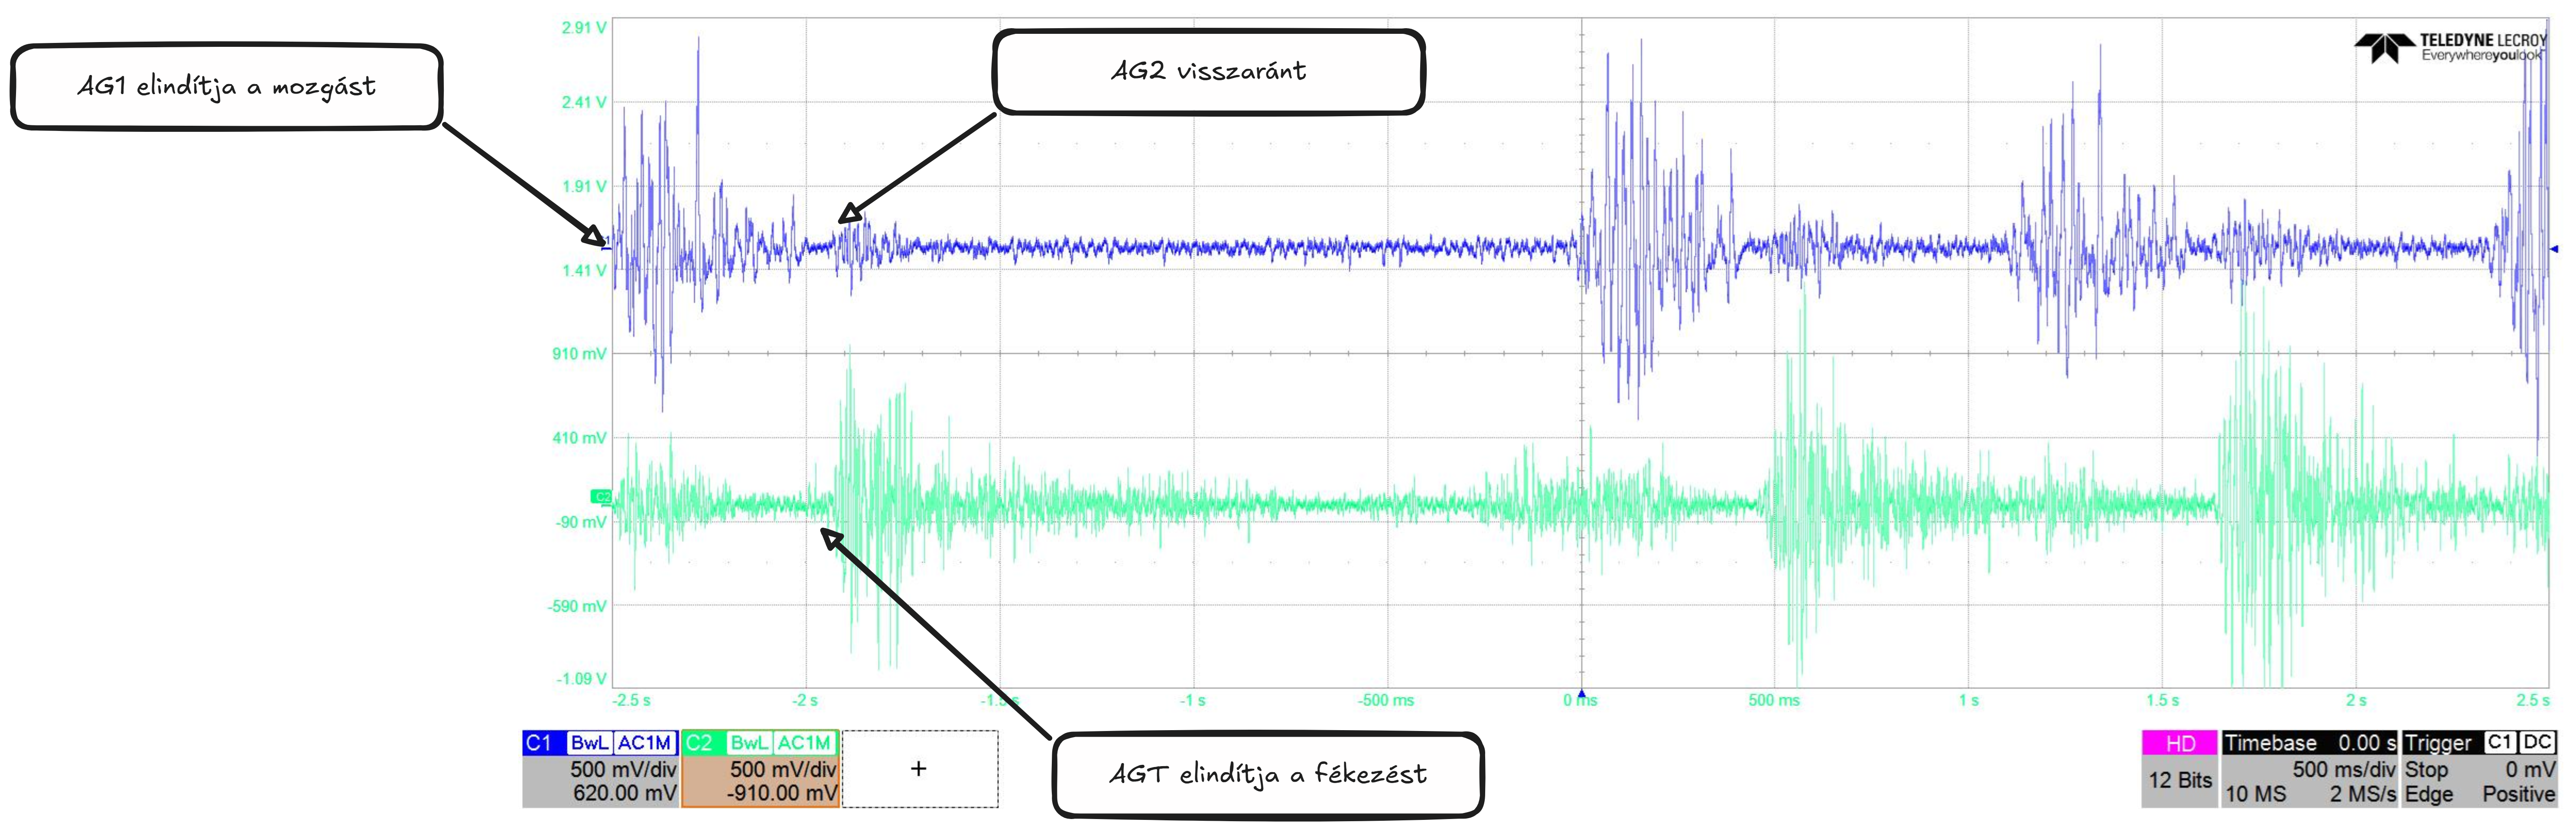
\includegraphics[width=\linewidth]{Images/palm-rotation.jpg}}
\caption{A tenyérforgató izmok trifázisos aktivitása.}
\label{fig:palm}
\end{figure}

A játék irányítása egy DualShock~4\texttrademark  \cite{DUALSHOCK4} kontroller gyorsulásmérőjével fog történni, a kontroller kormányként lesz fogva egy kézbe és az elforgatása lesz a felelős, mind a játék irányításáért, mind a trifázisos ballisztikos mozgásokért. 

\subsection{A micropython hiányosságai}

Sajnos rá kellett jönnünk, hogy a MicroPython interpreter overheadje okán nem volt képes elegendő mintavételi sebességet biztosítani mindkét szenzorhoz egyidejűleg, így az alábbi python kódot le kellett cserélnünk egy rust code-ra, amelyet ágensekkel segítségével hoztunk létre.

Azért választottuk rustot, mivel hardwerközeli nyelv, annyira hogy nem kell telepíteni a pico2-n semmit, mint a micropython esetében, csak átmásolni a bináris fájlt és már működik is. hardwerközeliségről lévén szó válaszhattunk volna más nyelvet is, mint mondjuk a C, C++, de mégis a rust mellett döntöttünk, mivel ez egy modernebb nyelv, ahol expliciten ki kell kapcsolnunk a biztonsági funkciókat, hogy olyan szabad memóriakezelésünk legyen mint a másik két említett nyelvben.
Az alábbi program binárisban küldi ki az adatokat számítógépre, ahol egy python scripttel fog történni a feldolgozás, ezt követi majd a játékmotor. 

\begin{figure}[H]
\centerline{
\includegraphics[width=\linewidth]{Images/technológiák.png}}
\caption{A tenyérforgató izmok trifázisos aktivitása.}
\label{fig:osszevetes}
\end{figure}




\begin{lstlisting}[language=Python]
import board
import analogbufio
import array
import ulab.numpy as np
import time
import usb_hid
import usb_cdc

# A csatlakoztatott USB HID eszközök közül kikeressük a gamepad-et.
# A gamepad Usage Page-e 0x01 (Generic Desktop), Usage-e 0x05 (Game Pad).
gamepad = None
for device in usb_hid.devices:
    if device.usage_page == 0x01 and device.usage == 0x05:
        gamepad = device
        break

# A HID report 7 bájtos: az első bájt a Report ID, a többi az adatmezők.
# A 4-es Report ID a custom gamepad descriptornak felel meg.
report = bytearray(7)
report[0] = 4

def send_integer(value):
    """Egyetlen értéket küld el az X tengely csatornaként (-127..127)."""
    report[3] = value & 0xFF
    gamepad.send_report(report)


# Egy-egy olvasási ciklus mintaszáma (100 minta / 1000 Hz = 100 ms ablak)
length = 100
buffer1 = array.array("H", [0x0000] * length)
buffer2 = buffer1[:]

# Mindkét ADC csatornát 1000 Hz-es mintavételi rátával inicializáljuk.
# GP26 = 1. szenzor (agonista izom), GP27 = 2. szenzor (antagonista izom)
rate = 1000
adcbuf1 = analogbufio.BufferedIn(board.GP26, sample_rate=rate)
adcbuf2 = analogbufio.BufferedIn(board.GP27, sample_rate=rate)

# A két csatorna nyers adatait tároljuk el utófeldolgozáshoz és kalibrációhoz.
data = []
calibration_data = []
start_time = None
minimal_activation_value = None

# Az interleaved küldési buffer: a két csatorna mintái felváltva kerülnek bele
# (combined[0], combined[2], ... = buffer1; combined[1], combined[3], ... = buffer2)
combined = np.zeros(len(buffer1) * 2, dtype=np.uint16)


try:
    while True:
        # Mindkét csatorna adatainak beolvasása a bufferekbe
        adcbuf1.readinto(buffer1)
        adcbuf2.readinto(buffer2)

        # Az adatokat interleaved formátumban fűzzük össze, majd elküldjük
        # a CDC adatcsatornán a PC-n futó vizualizációs programnak
        combined[0::2] = buffer1
        combined[1::2] = buffer2
        usb_cdc.data.write(combined.tobytes())

        # Az EMG aktivitás mértékét a szórással (std) becsüljük: nagyobb szórás
        # = erősebb izomaktivitás. Az arányuk adja a flow-értéket.
        value1 = np.std(np.array(buffer1))
        value2 = np.std(np.array(buffer2))
        if value2 != 0:
            value = value1 / value2
        else:
            value = 1.0
        data.append(value)

        # Az első iterációban rögzítjük a kezdőidőpontot
        if start_time is None:
            start_time = time.time()
        elapsed_time = round(time.time() - start_time)

        # Az első 3 másodperc a kalibrációs fázis: ekkor a felhasználó
        # relaxált állapotban van, az ekkor mért értékek adják az alapvonalat.
        if elapsed_time == 3:
            calibration_data = data[:]
            minimal_activation_value = min(calibration_data)

        # Kalibráció után összehasonlítjuk a jelenlegi értéket az alapvonallal
        # és ennek megfelelő HID jelet küldünk a játéknak.
        if elapsed_time > 3:
            if value >= minimal_activation_value:
                print(value)
                send_integer(120)
            else:
                print(value)
                send_integer(160)

        # A csúszóablak méretét 200 mintában korlátozzuk a memória kímélése érdekében
        if len(data) > 200:
            data.pop(0)


except Exception as e:
    print("CRASHED:", e)

finally:
    # Az ADC erőforrásokat mindig fel kell szabadítani leálláskor
    adcbuf1.deinit()
    adcbuf2.deinit()

\end{lstlisting}


\begin{lstlisting}[language=Rust]
#![no_std]
#![no_main]

use panic_halt as _;
use rp235x_hal as hal;
use cortex_m::singleton;
use hal::pac;
use hal::dma::{single_buffer, DMAExt};
use usb_device::{class_prelude::*, prelude::*};
use usbd_serial::SerialPort;

#[link_section = ".start_block"]
#[used]
pub static IMAGE_DEF: hal::block::ImageDef = hal::block::ImageDef::secure_exe();
// RP2350 külső kristályoszcillátor frekvenciája
const XTAL_FREQ_HZ: u32 = 12_000_000u32;

#[rp235x_hal::entry]
fn main() -> ! {
    let mut pac = pac::Peripherals::take().unwrap();
    let _core = cortex_m::Peripherals::take().unwrap();
    let mut watchdog = hal::Watchdog::new(pac.WATCHDOG);
    let clocks = hal::clocks::init_clocks_and_plls(
        XTAL_FREQ_HZ,
        pac.XOSC,
        pac.CLOCKS,
        pac.PLL_SYS,
        pac.PLL_USB,
        &mut pac.RESETS,
        &mut watchdog,
    )
    .unwrap();

    // SIO (Single-cycle I/O) blokk inicializálása -- szükséges a GPIO lábakhoz
    let sio = hal::Sio::new(pac.SIO);
    let usb_bus = UsbBusAllocator::new(hal::usb::UsbBus::new(
        pac.USB,
        pac.USB_DPRAM,
        clocks.usb_clock,
        true,
        &mut pac.RESETS,
    ));
    let mut serial = SerialPort::new(&usb_bus);
     let mut usb_dev = UsbDeviceBuilder::new(&usb_bus, UsbVidPid(0x16c0, 0x27dd))
        .strings(&[StringDescriptors::default()
            .manufacturer("HA8KDA")
            .product("Serial port")
            .serial_number("TEST")])
        .unwrap()
        .max_packet_size_0(64)
        .unwrap()
        .device_class(2)
        .build();

        // GPIO lábak inicializálása az IO_BANK0 perifériához
        let pins = hal::gpio::Pins::new(
            pac.IO_BANK0,
            pac.PADS_BANK0,
            sio.gpio_bank0,
            &mut pac.RESETS,
        );
        // DMA vezérlő inicializálása; a csatornák (ch0, ch1, ...) a split után érhetők el
        let dma = pac.DMA.split(&mut pac.RESETS);
        // ADC inicializálása; GP26 = 1. EMG csatorna, GP27 = 2. EMG csatorna
        let mut adc = hal::Adc::new(pac.ADC, &mut pac.RESETS);
        let mut adc_pin_0 = hal::adc::AdcPin::new(pins.gpio26.into_floating_input()).unwrap();
        let adc_pin_1 = hal::adc::AdcPin::new(pins.gpio27.into_floating_input()).unwrap();


    // Statikus DMA puffer: 1000 minta * 2 csatorna (round-robin), azaz 500 minta/csatorna
    let buf_for_samples = singleton!(: [u16; 1000] = [0; 1000]).unwrap();

        // ADC FIFO konfigurálása: 48 MHz / 48000 = 1000 Hz összesített mintavételi ráta,
        // round-robin 2 csatornán -> 500 Hz / csatorna; DMA-ra kapcsolva
        let mut adc_fifo = adc
        .build_fifo()
        .clock_divider(47999, 0)
        .set_channel(&mut adc_pin_0)
        .round_robin((&adc_pin_0, &adc_pin_1))
        .enable_dma()
        .start_paused();

        let mut dma_transfer = Some(
            single_buffer::Config::new(dma.ch0, adc_fifo.dma_read_target(), buf_for_samples).start()
        );
        adc_fifo.resume();
        let mut is_streaming = false;

        loop {
            // USB parancsok fogadása a PC-ről: 'W'/'w' = adatfolyam indítása, 'X'/'x' = leállítása
            if usb_dev.poll(&mut [&mut serial]) {
                let mut rx_buf = [0u8; 8];
                if let Ok(count) = serial.read(&mut rx_buf) {
                    for i in 0..count {
                        match rx_buf[i] as char {
                            'W' | 'w' => is_streaming = true,
                            'X' | 'x' => is_streaming = false,
                            _ => {}
                        }
                    }
                }
            }

            // Ha a DMA átvitel befejezte a puffer feltöltését, feldolgozzuk az adatokat
            if dma_transfer.as_ref().map_or(false, |t| t.is_done()) {
                let transfer = dma_transfer.take().unwrap();
                // A wait() lezárja az átvitelt és visszaadja a DMA csatornát,
                // az ADC olvasási célpontot és a mintapuffert újrafelhasználáshoz
                let (ch, adc_read_target, buf) = transfer.wait();

                if is_streaming {
                    // A u16 mintákat nyers bájtokként küldjük el (little-endian, 2 bájt/minta)
                    let raw_ptr = buf.as_ptr() as *const u8;
                    let byte_len = buf.len() * 2;
                    let bytes = unsafe { core::slice::from_raw_parts(raw_ptr, byte_len) };

                    let mut written = 0;
                    while written < bytes.len() {
                        if let Ok(n) = serial.write(&bytes[written..]) {
                            written += n;
                        } else {
                            break;
                        }
                    }
                }

                /* Új DMA átvitel indítása ugyanazokkal az erőforrásokkal -- körkörösen fut */
                dma_transfer = Some(
                    single_buffer::Config::new(ch, adc_read_target, buf).start()
                );
            }




        }
}



/// Program metadata for `picotool info`
#[link_section = ".bi_entries"]
#[used]
pub static PICOTOOL_ENTRIES: [hal::binary_info::EntryAddr; 5] = [
    hal::binary_info::rp_cargo_bin_name!(),
    hal::binary_info::rp_cargo_version!(),
    hal::binary_info::rp_program_description!(c"USB Serial Example"),
    hal::binary_info::rp_cargo_homepage_url!(),
    hal::binary_info::rp_program_build_attribute!(),
];




\end{lstlisting}

\subsection{A Flow score}

A külső témavezetőmmel való konzultáció során arra jutottunk, hogy az alábbi értékek fognak kelleni a flow score kiszámításához:

\begin{itemize}
    \item Agonista és Antagonista amplitúdójának az aránya
    \item Agonista és antagonista izmok koaktivációja.
\end{itemize}

\subsubsection{Agonista és Antagonista amplitúdójának az aránya}

Az amplitúdó-arány (magnitude ratio) – amely az agonista és antagonista EMG-jelek integrált területének (AUC) hányadosaként definiálható – a motoros rendszer hatékonyságának egyik kulcsmutatója. Ha az agonista dominánsan, de arányosan nagyobb amplitúdóval aktiválódik az antagonistához képest, az arra utal, hogy a központi idegrendszer pontosan kalibrálta az erőkifejtést: elegendő impulzust ad a mozgás indításához, miközben az antagonista fékezés mértéke éppen annyi, amennyi a végpont pontos eléréséhez szükséges. \cite{amplitude1} Ezzel szemben, ha az antagonista amplitúdója aránytalanul magas az agonistához képest, az kompenzációra utalhat, ami rontja a mozgás folyamatosságát\cite{amplitude2}


\subsubsection{Agonista és antagonista izmok koaktivációja}

A flow állapot egyik biomechanikai predikátora a motoros hatékonyság, ezt a szakirodalom az agonista és antagonis izmok egyidejű feszülésének csökkenésével írja le. A gyakorlott, célorientált cselekvések során a központi idegrendszer olyan pontosan kalibrálja a mozdulatot indító erőkifejtést, hogy kevesebb korrekcióra és mérsékeltebb antagonista "fékezésre" van szükség a végtag pontos megállításához.\cite{coactivation2,coactivation3,coactivation5, coactivation4}










\section{A játék}

\subsection{Követelmények}

Cél: Általános koncentrációs képességek javítása

\begin{itemize}
    \item legyünk képesek beolvasni a flow score-t
    \item a flow score-hoz igazodjon a játék sebessége
    \item a flow score-hoz igazodjon az akadályok mennyisége
    \item legyen 10 előre megadott nehézségi szintű pálya, amelyek helye teljesítési útvonalának abszolút hossza azonos
    \item figyelje hányszor hibázik a játékos és csökkentse a nehézséget (sebesség + akadályok mennyisége)
    \item hibátlan teljesítmény esetén növekedjen a nehézség, a (plafon - 1)-igaznak
    \item go és no go ingerek váltogatása
    \item 
    \item 
\end{itemize}

\subsection{Valós idejű jelfeldolgozás és hálózati zajszűrés}

Az sEMG mérések során a környezeti elektromos hálózatból származó 50\,Hz-es zaj \textit{(power-line interference)} jelentősen torzíthatja a jelszinteket. Mivel a Flow Score számításban kulcsszerepet játszik az agonista és antagonista jelek görbe alatti területe (AUC) és azok metszete, a zajból adódó állandó oszcilláció a szoftverben hamis -- a valóságnál nagyobb -- területi értékeket, ezáltal hibás koaktivációs indexet (CAI) eredményezne.

Ennek elkerülésére a Python alapú feldolgozó komponensben (\texttt{szabi.py}) a beérkező és csúszóablakban (sliding window) tárolt nyers adatsorokon egy digitális IIR lyukszűrőt (Notch filter) alkalmazunk $50\,$Hz-es középfrekvenciával és $Q=30$ jósági tényezővel. A megvalósítás során a \texttt{scipy.signal} könyvtár \texttt{iirnotch} és \texttt{filtfilt} metódusait hívjuk meg. Kiemelendő a \texttt{filtfilt} használata, amely a szűrést előrefelé és hátrafelé is elvégzi az adatsoron: ez az úgynevezett nulla fázistolású (zero-phase) szűrés garantálja, hogy a zajcsökkentés nem okoz időbeli késleltetést vagy fáziseltolódást a két izomcsatorna jelei között, így a koaktiváció (egymásra feszítés) időbeli egybeesése mérnökileg pontos marad. A szűrt adatok ezután kerülnek át a \texttt{calc\_magnitude\_ratio} és \texttt{calc\_reciprocal\_efficiency} algoritmusokba.

\subsection{A játékmotor}

A godot játékmotorra esett végül a választásunk \cite{godot_engine}, ennek elsődleges oka a unity-vel szemben a godot sokkal kezdőbarátabb és nem csak C\#-ban lehet benne szkripteket írni hanem a pythonos godot scriptben is. A godot barátságosságát érzékelteti az is, hogy egy darab portable exe futtatása elengedő hozzá, nincs hosszú telepítési idő, több gigabájtos telepítés, de mégis rendelkezik minden szükséges fejlesztési eszközzel, amire szükségünk lehetett.  \clearpage
\section{Mikroműholdak bemutatása}
Az űrtechnológia fejlődésével egyértelművé vált az ipar számára, hogy olyan szakemberekre van szükség a nagy projektekhez, akik már gyakorlottak legalább minimális szinten a műholdfejlesztés folyamatainak egy részében. A 2000-es évek elején Robert Twiggs, amerikai professzor javaslatára egységes méret-rendszert hoztak létre a kis műholdak számára. Így alakult ki a Twiggs-elv, mely alapján az egységnyi kis műhold mérete $10cm\times10cm\times10cm$, tömege maximum $1kg$. A kialakításból adódóan ezeket CubeSat-nek kezdték el becézni. Mivel egységnyi méretet szabtak meg, így könnyen skálázhatóvá vált, hogy mekkora mikroműholdat lehet készíteni adott célra.

Szakdolgozatom témájaként egy ilyen CubeSat műhold fedélzeti számítógépét kezdtem el fejleszteni hardvertől szoftverig. A folyamat során inspirált az elérni kívánt cél, a már meglévő magyar sikerek és a mikrovezérlők programozása iránti kíváncsiságom is~\cite{masat-origo}.

\subsection{Modulok egy CubeSat műholdon}
Egy CubeSat műholdnak több felépítő egysége van, melyek közül kritikus elemek a kommunikációs modul, az energiaellátásért felelős napelemek és tápegység, illetve a mindent összekötő fedélzeti számítógép (OBC = On Board Computer).

Mindezek mellett szükséges minimum egy, valamiféle kísérletet vagy egyéb funkcionalitást megvalósító egység is annak érdekében, hogy ne csak kommunikálni lehessen a műholddal, hanem 
legyen valami haszna is. %Úgy írnám, hogy rentábilis legyen. Szeretem a kőművesnyelvet és művelem is, egy szakdoga ennél egy hajszállal (nem többel) fennköltebb.
Mivel szakdolgozatomban az OBC-vel foglalkoztam, így azon modult fejtem ki jobban a következőekben.

%Ide jobban ki lehetne fejteni, akár egy szép ábrával, hogy mik vannak egy műholdban, mikkel kommunikál egy OBC.

\Aref{fig:obcfeladatok}. ábra foglalja össze a legfőbb feladatokat.

\begin{figure}
        \centering
        \begin{adjustbox}{width=\textwidth} % Scale the forest to fit text width
\begin{forest}
for tree={
  grow'=south, % Children grow downwards
  align=center, % Center-align text in nodes
  edge path={
    \noexpand\path [draw, \forestoption{edge}] (!u.parent anchor) -- (.child anchor)\forestoption{edge label};
  },
  inner sep=2pt, % Padding inside nodes
  l sep+=0.5cm, % Vertical spacing between levels
  s sep+=0.5cm % Horizontal spacing between siblings
}
[On-Board Computer
  [Kommunikáció
    [Csomagküldtés
      [Csomagküldtés
        [Csomagküldtés]
      ]
      [Csomagküldtés
        [Csomagküldtés]
      ]
    ]
    [Trials during the test
      [Appearance of the stimuli
        [Time series for each epoch]
      ]
      [Answer to the stimuli
        [Time series for each epoch]
      ]
    ]
  ]
  [Recordings from the  test
        [\{\ldots\}]
  ]
]
\end{forest}
\end{adjustbox}
        \caption{Az OBC feladatai}
        \label{fig:obcfeladatok}
\end{figure}



\section{Fedélzeti számítógép}
A fedélzeti számítógép a lelke minden űreszköznek, akárcsak az újabb gépjárműveknek~is.

Az OBC időzíti a perifériák működését, ellenőrzi azok működőképességét és felel a műhold moduljainak összhangban tartásáért. Mindezek mellett adatokat gyűjt, melyek alapján optimalizálni lehet a működést, későbbi küldetésekhez szerezhetnek a fejlesztők/kutatók további információkat.

\subsection{Fejlesztéshez szükséges eszközök}
A fejlesztés két nagyobb fázisra bontható szét. Az első fázisban a hardvert kellett megtervezni, melyhez a KiCad~8.0~\cite{kicad} ingyenes tervezőprogramot használtam. Miután megérkeztek az alkatrészek és a lész nyomtatott áramkör, kézi forrasztással helyére illesztettem az alkatrészeket. Az áramkör \aref{fig:kapcsolasi_rajz}.~ábrán látható.

\subsubsection{Nyomtatott áramkör fejlesztése}

 \clearpage

\section*{Nyilatkozat}
\noindent
Alulírott \theauthor, programtervező informatikus szakos hallgató, kijelentem, hogy a dolgozatomat a Szegedi Tudományegyetem, Informatikai Intézet Műszaki Informatika Tanszékén készítettem, BSc diploma megszerzése érdekében.
%TODO tanszek es diplomahoz valami
Kijelentem, hogy a dolgozatot más szakon korábban nem védtem meg, saját munkám eredménye, és csak a hivatkozott forrásokat (szakirodalom, eszközök stb.) használtam fel.

Tudomásul veszem, hogy szakdolgozatomat a Szegedi Tudományegyetem Diplomamunka Repozitóriumában tárolja.

\vspace*{2cm}

\begin{tabular}{lc}
Szeged, \today\
\hspace{2cm} & \makebox[6cm]{\dotfill} \\
& aláírás \\
\end{tabular} \clearpage

%\section*{Köszönetnyilvánítás}
%
%Ezúton szeretnék köszönetet mondani \textbf{X. Y-nak} ezért és ezért \ldots
%
%\clearpage

%Opcionális rész. Ichletat adó együttes/zenész, család, barátok stb. Esetleg az egyetemenk, amiért biztosította az eszközöket. Egyéb egyetemi munkatársak, közösségek. \clearpage
\section{License}

This thesis is licensed under a 
\href{https://creativecommons.org/licenses/by-nc/4.0/}{Creative Commons Attribution-NonCommercial 4.0 International License (CC-BY-NC)}. 

You are free to share and adapt the material under the following terms:
\begin{itemize}
  \item Attribution: You must give appropriate credit, provide a link to the license, and indicate if changes were made.
  \item NonCommercial: You may not use the material for commercial purposes.
\end{itemize}

For additional details, please refer to the full license at 
\url{https://creativecommons.org/licenses/by-nc/4.0/}.

 \clearpage

\begingroup %hivatkozásjegyzék
\sloppy


\printbibliography[heading=bibintoc]
\endgroup
\clearpage %hivatkozásjegyzék vége

\section*{Függelék}

\begin{landscape}
\begin{figure}
    \centering
    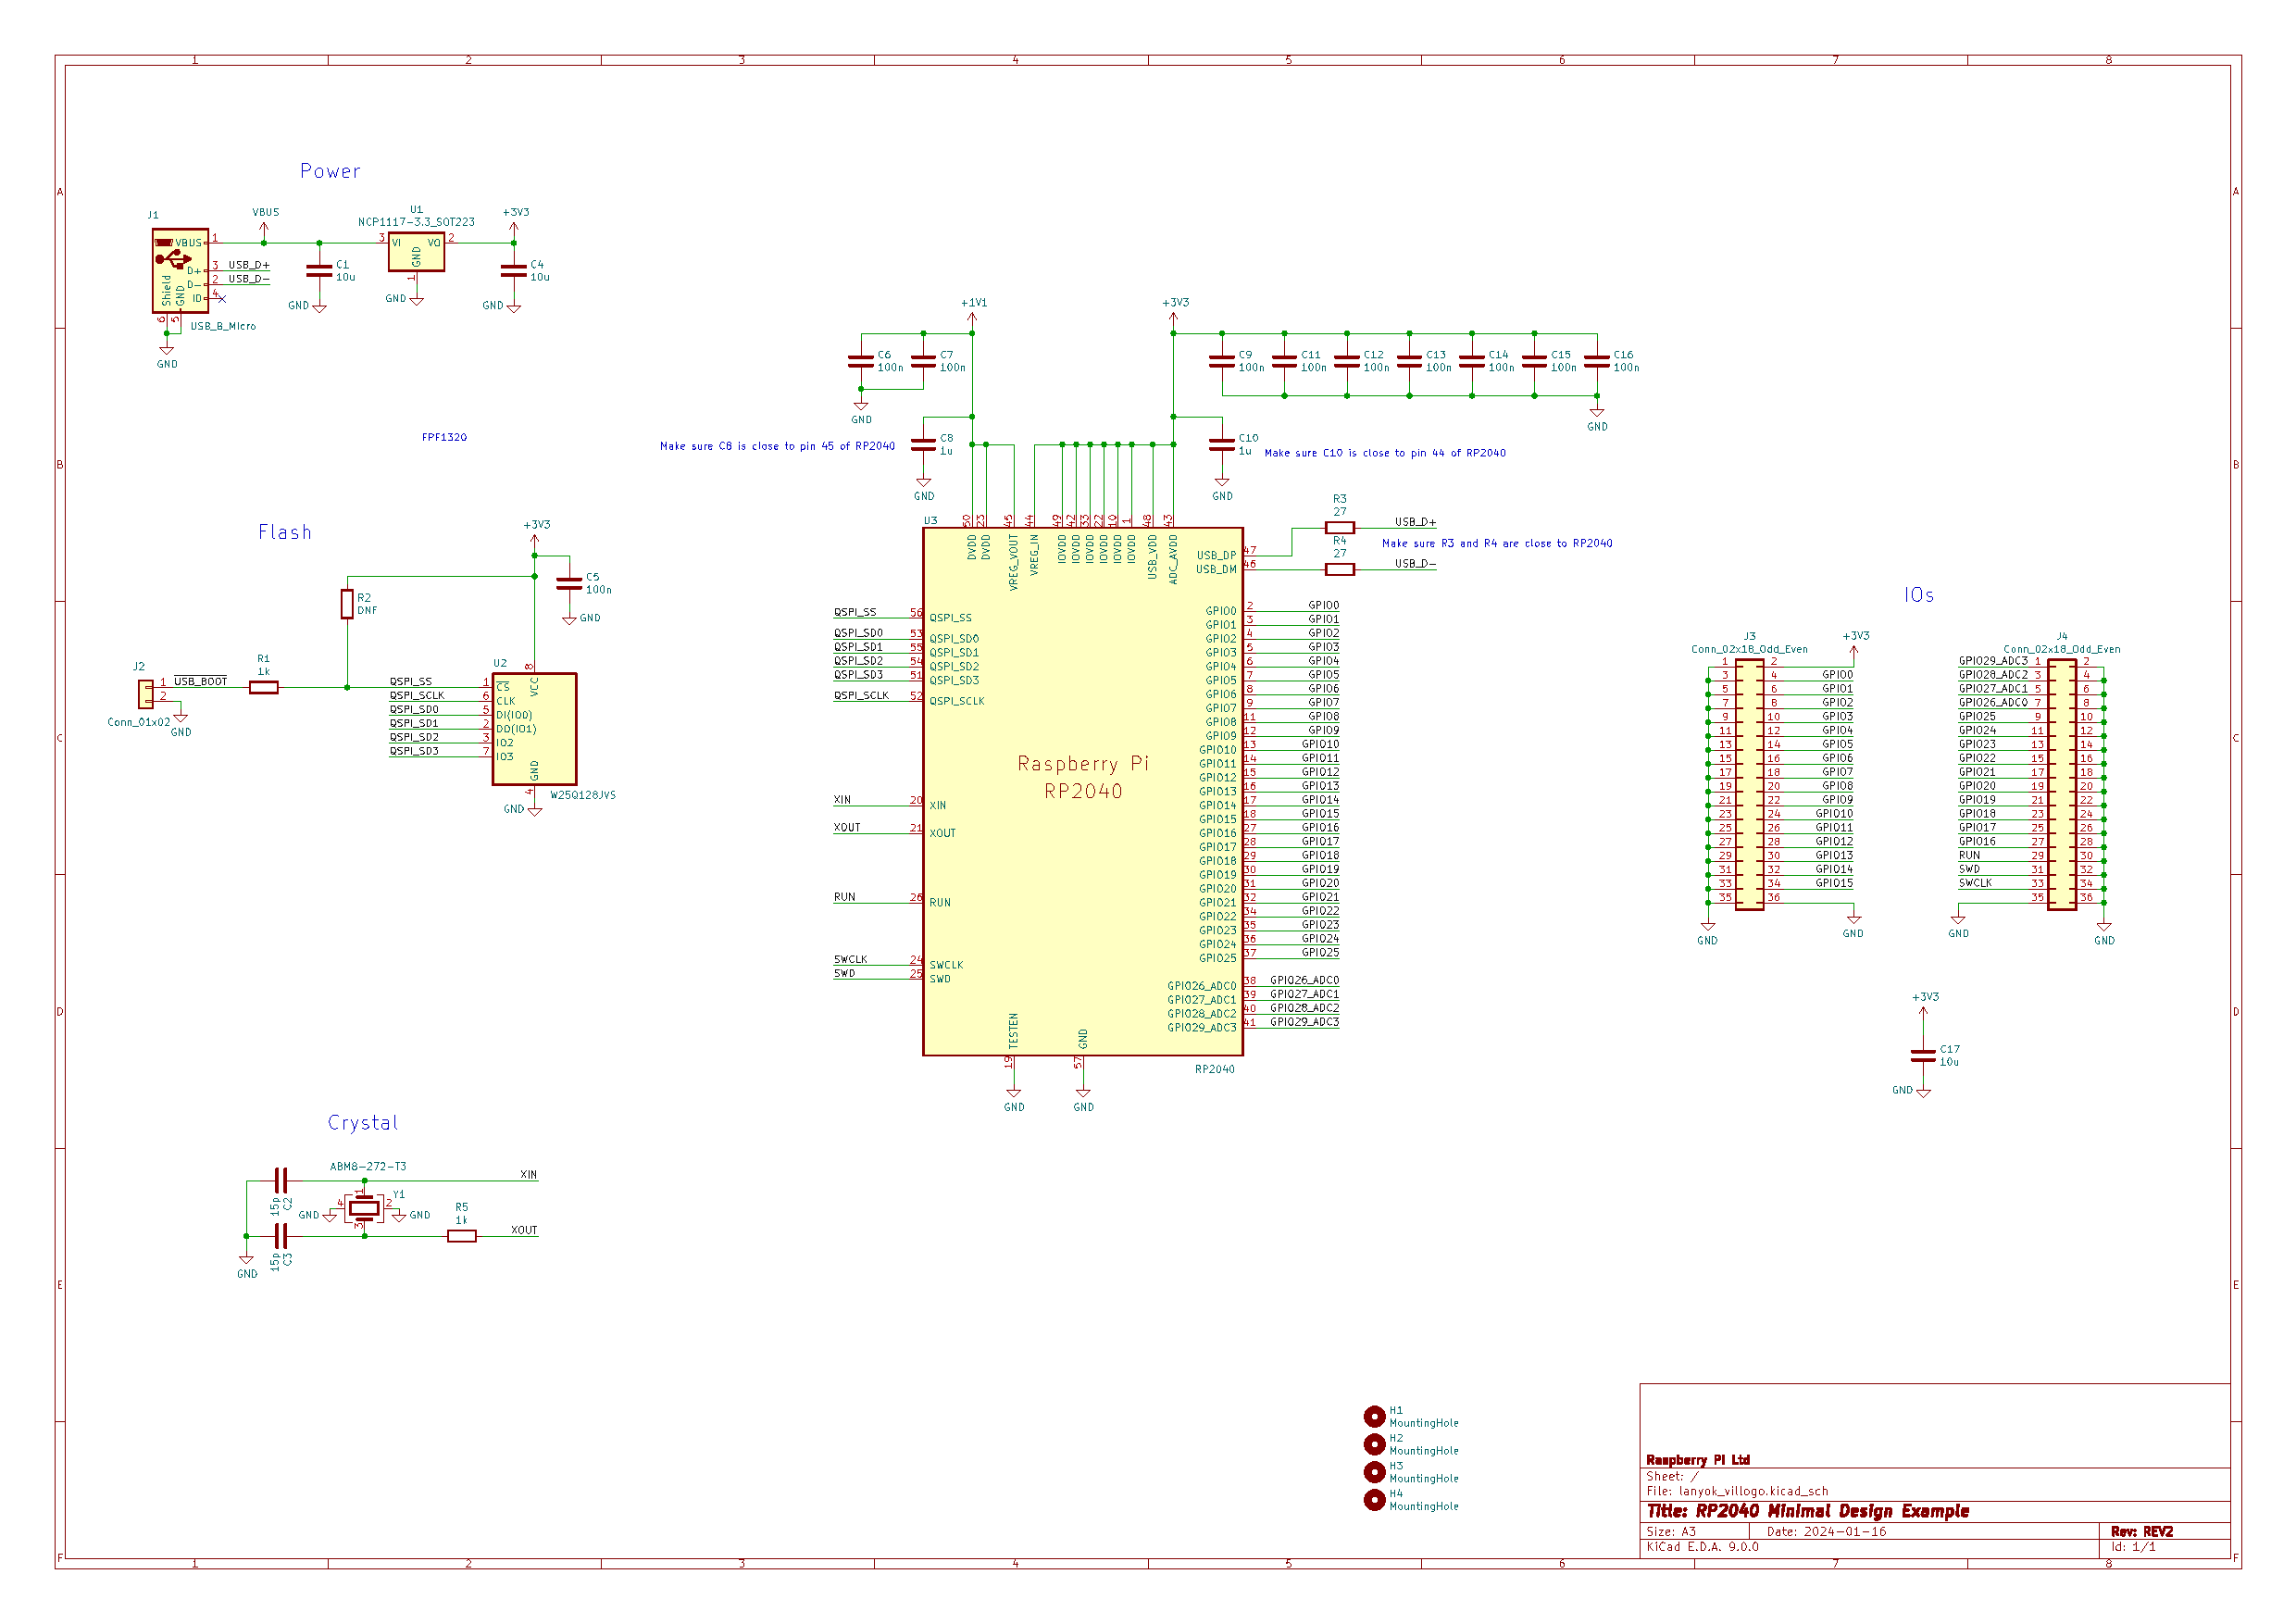
\includegraphics[width=0.8\linewidth]{schematic1.pdf}
    \caption{Kapcsolási rajz PÉLDA; KiCAD --> Plot --> pdf}
    \label{fig:kapcsolasi_rajz}
\end{figure}

\end{landscape}

\subsection*{A program forráskódja}
A függelékbe kerülhetnek a hosszú táblázatok, vagy mondjuk egy programlista:



\end{document}